\documentclass[a4paper, 11pt, twoside]{report}

\usepackage[T1]{fontenc}
\usepackage[utf8]{inputenc}
\usepackage[french]{babel}
\usepackage{newpxtext,newpxmath} 
\usepackage{microtype}
\usepackage{xcolor}
\usepackage{titlesec}
\usepackage{geometry}
\usepackage{dsfont}
\usepackage{graphicx}
\usepackage{amsthm}
\usepackage{enumitem}
\usepackage{fancyhdr} % Pour les en-têtes
\usepackage{titletoc}
\usepackage[most]{tcolorbox} % Monté ici pour centraliser les packages

\geometry{a4paper, top=3cm, bottom=3cm, inner=3cm, outer=2.5cm, headheight=14pt}

% --- Palette de Couleurs "Deep Academic" ---
\definecolor{MainBlue}{RGB}{20, 50, 90}      % Bleu Nuit (Titres)
\definecolor{SecondaryBlue}{RGB}{40, 90, 140} % Bleu Moyen
\definecolor{DefColor}{RGB}{0, 100, 80}      % Vert Émeraude sombre (Définitions)
\definecolor{PropColor}{RGB}{140, 30, 30}    % Rouge Sombre (Propositions)
\definecolor{ExoColor}{RGB}{100, 60, 0}      % Ambre brûlée (Exercices)
\definecolor{RemColor}{RGB}{80, 80, 80}      % Gris de Payne (Remarques)

% --- Style des Chapitres (Plus moderne) ---
\titleformat{\chapter}[display]
  {\normalfont\huge\bfseries\color{MainBlue}}
  {\filleft\Large\textsf{\chaptertitlename} \Huge\thechapter}
  {1ex}
  {\titlerule[1.5pt]\vspace{1ex}\filright}
  [\vspace{1ex}\titlerule]

% --- Configuration des Titres de sections ---
\titleformat{\section}{\normalfont\Large\bfseries\color{MainBlue}}{\thesection}{1em}{}
\titleformat{\subsection}{\normalfont\large\bfseries\color{SecondaryBlue}}{\thesubsection}{1em}{}

% --- En-têtes et Pieds de page ---
\pagestyle{fancy}
\fancyhf{}
\fancyhead[RO,LE]{\small\color{gray}\textsf{\thepage}}
\fancyhead[LO]{\small\color{gray}\textsf{\rightmark}}
\fancyhead[RE]{\small\color{gray}\textsf{\leftmark}}
\renewcommand{\headrulewidth}{0.2pt}
\addtolength{\headwidth}{0pt}

% --- Personnalisation des listes ---
\setlist[itemize,1]{label=\color{SecondaryBlue}$\bullet$}
\setlist[enumerate,1]{label=\color{SecondaryBlue}\arabic*)}

% ==============================================================
% --- COMPTEURS (Nouveau) ---
% Compteur partagé pour tout sauf les exercices
\newcounter{envcpt}[chapter]
\renewcommand{\theenvcpt}{\thechapter.\arabic{envcpt}}

% Compteur spécifique pour les exercices
\newcounter{exocpt}[chapter]
\renewcommand{\theexocpt}{\thechapter.\arabic{exocpt}}
% ==============================================================

% --- Environnements SANS CADRES (Amélioration typographique + Comptage) ---

\newenvironment{definition}[1][]{
    \medskip\par\noindent\refstepcounter{envcpt}
    % Ici on a remplacé \ --- #1 par \ (#1) pour avoir des parenthèses
    \textcolor{DefColor}{\rule[0pt]{2pt}{10pt}\hspace{0.5em}\textbf{Définition \theenvcpt \ifx&#1&\else\ (#1)\fi.}} \itshape
}{
    \par\medskip
}

\newenvironment{proposition}[1][]{
    \medskip\par\noindent\refstepcounter{envcpt}
    % Ajout de l'option [#1] pour pouvoir nommer les propositions aussi
    \textcolor{PropColor}{\rule[0pt]{2pt}{10pt}\hspace{0.5em}\textbf{Proposition \theenvcpt \ifx&#1&\else\ (#1)\fi.}} \itshape
}{
    \par\medskip
}

\newenvironment{lemme}[1][]{
    \medskip\par\noindent\refstepcounter{envcpt}
    \textcolor{PropColor}{\rule[0pt]{2pt}{10pt}\hspace{0.5em}\textbf{Lemme \theenvcpt \ifx&#1&\else\ (#1)\fi.}} \itshape
}{
    \par\medskip
}

\newenvironment{exemple}[1][]{
    \medskip\par\noindent\refstepcounter{envcpt}
    \textcolor{RemColor}{\small\textbf{\textsf{Exemple \theenvcpt \ifx&#1&\else\ (#1)\fi.}}} 
}{
    \par\medskip
}

\newenvironment{remarque}[1][]{
    \medskip\par\noindent\refstepcounter{envcpt}
    \textcolor{RemColor}{\small\textbf{\textsf{Remarque \theenvcpt \ifx&#1&\else\ (#1)\fi.}}} 
}{
    \par\medskip
}

\newenvironment{exercice}[1][]{
    \medskip\par\noindent\refstepcounter{exocpt}
    \textcolor{ExoColor}{\textbf{\small\scshape Exercice \theexocpt \ifx&#1&\else\ (#1)\fi.}} \small
}{
    \par\medskip
}

% --- Théorème (Lié au compteur partagé) ---
% --- Théorème (Lié au compteur partagé) ---
% L'ajout du DEUXIÈME [] est crucial ici pour rendre l'argument optionnel !
\newtcolorbox[use counter=envcpt]{theoreme}[1][]{
    enhanced, sharp corners, boxrule=0.8pt,
    colback=white, colframe=MainBlue,
    fonttitle=\bfseries, coltitle=MainBlue,
    title={Théorème \thetcbcounter \ifx&#1&\else\ (#1)\fi},
    attach title to upper={\textbf{. }},
}

% --- Preuve avec fin de démo stylisée (et support du titre personnalisé) ---
% L'ajout du [1][Démonstration] permet de changer le mot par défaut
\renewenvironment{proof}[1][Démonstration]{
    \par\noindent \textit{\small #1.} 
}{
    \hfill \textcolor{MainBlue}{$\blacksquare$} \par\medskip
}

% --- Macros Mathématiques ---
\newcommand{\R}{\mathbb{R}}
\newcommand{\N}{\mathbb{N}}
\newcommand{\Z}{\mathbb{Z}}
\newcommand{\Prob}{\mathbb{P}}
\newcommand{\Esp}{\mathbb{E}}
\newcommand{\ind}{\mathds{1}}

% --- Page de garde améliorée ---
\newcommand{\makecoursepage}{
    \begin{titlepage}
        \centering
        \vspace*{3cm}
        {\large \textsc{\color{gray} Université de Mons} \par}
        \vspace{1cm}
        \rule{\linewidth}{0.5pt} \\ [0.4cm]
        {\Huge \bfseries \color{MainBlue} Probabilité 1 \par}
        \rule{\linewidth}{2pt} \\ [1cm]
        {\Large \textsf{Notes de cours} \par}
        \vspace{2cm}
        {\Large Piette Tiago \par}
        \vfill
        {\small \textsf{Bac 2 Mathématiques} \par}
        {\small \textsf{Année académique 2025-2026} \par}
    \end{titlepage}
}

% ==============================================================
% PACKAGES DE LIENS ET RÉFÉRENCES (TOUJOURS À LA FIN DU PRÉAMBULE)
\usepackage[hidelinks]{hyperref} % Rend la table des matières cliquable
\usepackage[french]{cleveref} % Pour les références intelligentes (\cref)
% ==============================================================
\newcommand{\alors}{\Rightarrow}
\newcommand{\partie}{\mathcal{P}}
\newcommand{\interoo}[1]{\left] #1\right[}  % ]a,b[
\newcommand{\interof}[1]{\left] #1\right]}   % ]a,b]
\newcommand{\interfo}[1]{\left[ #1\right[}   % [a,b[
\newcommand{\interff}[1]{\left[ #1\right]}   % [a,b]
\newcommand{\fonction}[3]{#1\colon \left\{\begin{array}{l}#2 \\#3\end{array}\right.}
\newcommand{\A}{\mathscr{A}}
\usepackage{centernot}
\newcommand{\indep}{\mathrel{\perp\!\!\!\perp}}
\newcommand{\nindep}{\centernot\indep}
\newenvironment{notation}{
    \medskip\par\noindent
    \textcolor{RemColor}{\small\textbf{\textsf{Notation.}}} 
}{
    \par\medskip
}
\newcommand{\E}{E}
\newcommand{\Cov}{\operatorname{Cov}}
\newcommand{\Var}{\operatorname{Var}}
\usepackage[table]{xcolor}

% Pour les couleurs dans la matrice

% --- Couleurs personnalisées ---
\definecolor{diagblue}{RGB}{230, 230, 255}
\definecolor{covgreen}{RGB}{230, 255, 230}
\usepackage{tikz}
\usetikzlibrary{arrows.meta, positioning}
\begin{document}

\definecolor{encre}{RGB}{28,28,30}
\definecolor{accent}{RGB}{90,110,140}
\begin{titlepage}
\thispagestyle{empty}

% ---------- Filigrane : le cercle d'Apollonius ----------
\begin{tikzpicture}[remember picture, overlay]
  \node[opacity=0.16] at ($(current page.center)+(0,-0.6cm)$)
    {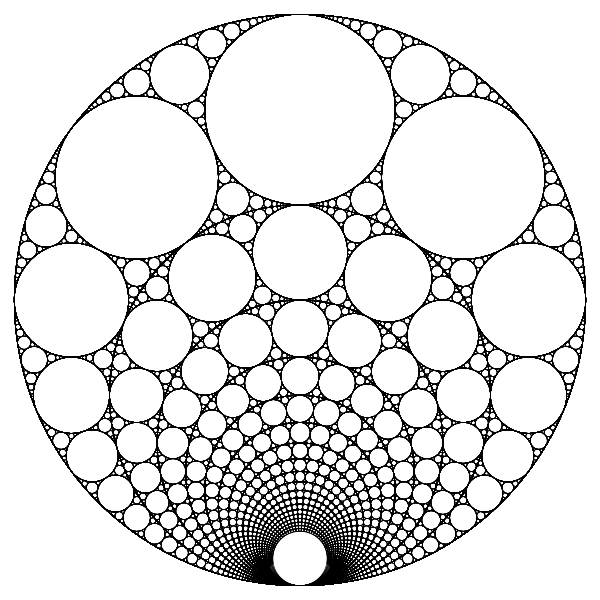
\includegraphics[width=17cm]{apollonius.png}};
\end{tikzpicture}

% ---------- Contenu ----------
\begin{center}
\vspace*{2.2cm}

{\footnotesize\color{accent}\scshape\selectfont
 \setlength{\baselineskip}{1.6em}
 Université de Mons \quad$\cdot$\quad Faculté des Sciences\par}

\vspace{3.4cm}

{\color{accent}\rule{2.2cm}{0.8pt}}

\vspace{1.1cm}

{\fontsize{43}{50}\selectfont\color{encre}
 Probabilités\,\textsc{\,i}\par}

\vspace{1.0cm}

{\large\color{encre} Notes de cours\par}

\vspace{0.9cm}

{\color{accent}\rule{2.2cm}{0.8pt}}

\vfill

{\normalsize\color{encre}\scshape Hamiot Manoa -- Piette Tiago\par}
\vspace{0.35cm}
{\footnotesize\color{accent}BaB3 --- Sciences mathématiques\par}
\vspace{0.15cm}
{\footnotesize\color{accent}2026\,--\,2027\par}

\vspace{1.4cm}
\end{center}

\end{titlepage}


\tableofcontents

\chapter{Axiomatique et calcul des probabilités}
\section{Introduction}

\section*{Introduction aux Probabilités}

Les probabilités constituent un domaine des mathématiques visant à modéliser et quantifier l'incertitude inhérente à certains phénomènes, qu'ils soient naturels, expérimentaux ou abstraits. Intuitivement, on cherche à associer à chaque \og événement possible \fg{} un nombre compris entre $0$ et $1$ reflétant notre degré de confiance en sa réalisation.

\medskip 

Formaliser rigoureusement cette idée n'est cependant pas immédiat : la théorie moderne des probabilités repose sur la \textbf{théorie de la mesure} et des résultats analytiques qui n'ont pas encore été vus. Un traitement pleinement rigoureux exigerait donc de maîtriser l'\textbf{intégrale de Lebesgue} et la théorie de la mesure, outils qui dépassent le cadre de ce cours. 

\medskip

C'est pourquoi nous adopterons ici une approche volontairement informelle : nous travaillerons principalement sur des espaces de probabilité discrets ou continus simples, en admettant certains résultats analytiques sous-jacents, tout en conservant la rigueur propre aux mathématiques dans les définitions, les énoncés et les démonstrations.

Nous allons alors introduire la notion suivante :

\begin{definition}
    Une \emph{expérience aléatoire} est une expérience dont on connaît l'ensemble des résultats possibles, mais dont le résultat effectif dépend du hasard.
\end{definition}

\begin{notation}
    On note $\Omega$ l'ensemble des résultats possibles de l'expérience aléatoire.
\end{notation}

\begin{exemple} 
    Voici quelques exemples d'expériences aléatoires et de l'ensemble $\Omega$ associé :
    \begin{itemize}
        \item Lancer d'un dé : $\Omega=\{1,2,3,4,5,6\}$. \label{ex:lancer_de}
        \item Lancer de deux pièces : $\Omega= \{(P,P),(P,F),(F,P),(F,F)\}$.
        \item Durée de vie d'une machine : $\Omega = [0,+\infty[$.
    \end{itemize} 
\end{exemple}

\begin{definition}
    Un \emph{événement} est un sous-ensemble des résultats possibles, dont on veut mesurer les chances de réalisation.
\end{definition}

Par exemple, dans le lancer d'un dé (cf. exemple \ref{ex:lancer_de}), on peut définir les événements suivants : $A= \{4\}$ (le résultat est 4), $B= \{1,2,3,4\}$ (le résultat est inférieur ou égal à 4) et $C= \{2,4,6\}$ (le résultat est pair).

\begin{definition}
    On appelle \emph{résultat} (ou issue) le choix d'un élément $\omega\in\Omega$. On dit qu'un événement $A$ est \emph{réalisé} si le résultat $\omega$ appartient à $A$.
\end{definition}

\begin{definition}[approche intuitive]
    Une \emph{mesure de probabilité} est une application 
    \[
    \fonction{P}{\mathcal{A}\to [0,1]}{A \in \partie (A)}
    \]
    où $P(A)$ représente la vraisemblance (ou la chance) que l'événement $A$ se réalise lors de l'expérience, et où $\mathcal{A}$ est l'ensemble des événements.
\end{definition}

Informellement, on interprète $P(A)= 1$ comme le fait que $A$ est certain de se réaliser. Si $P(A)=0$, nous sommes certains que $A$ ne se réalisera pas. Enfin, $P(A)= 0{,}37$ signifie que l'événement $A$ a $37\,\%$ de chances de se réaliser.

Pour calculer $P(A)$, on peut imaginer réaliser $N$ fois l'expérience aléatoire (de manière indépendante) et noter $P_N(A) = \frac{\#\{\text{fois où } A \text{ s'est réalisé}\}}{N}$. On définit alors naïvement la probabilité par passage à la limite :
\[
P(A)= \lim_{N\to +\infty}P_N(A).
\]

\begin{proposition}
    Si $\Omega$ est un ensemble fini et que tous les résultats sont équiprobables, alors :
    \[
    \forall A\in \mathcal{A} \quad P(A) = \frac{\# A}{\#\Omega}.
    \]
\end{proposition}

\begin{remarque}
    Soient $A$ et $B$ des événements. On est souvent amené à considérer les événements composés suivants :
    \begin{itemize}
        \item $A\cup B$ : [$A$ se réalise ou $B$ se réalise] ;
        \item $A\cap B$ : [$A$ se réalise et $B$ se réalise] ;
        \item $A^c$ : [$A$ ne se réalise pas].
    \end{itemize}
\end{remarque}

Il est clair au vu de cette première approche des probabilités d'événements équiprobables que, en pratique, la notion de dénombrement est essentielle. Nous allons voir, dans la section suivante, des outils fort pratiques pour dénombrer un ensemble.

\section{Combinatoire}

L’analyse combinatoire est l’art de compter les éléments d’ensembles finis. Elle est donc cruciale pour calculer des probabilités dans le cas d’équiprobabilité.

\begin{proposition}[Principe fondamental du dénombrement]
    Si l'on considère $k$ expériences $E_1,\dotsc,E_k$ telles que chaque expérience $E_j$ possède $r_j$ résultats possibles, alors le nombre total de résultats possibles pour la suite d'expériences $(E_1,\dots,E_k)$ est donné par le produit $r_1 \cdot r_2 \dotsm r_k$.
\end{proposition}

Le résultat s’effectue sans difficulté par récurrence.

 \begin{exemple}
     Si une personne possède $3$ pulls, $2$ pantalons et $10$ paires de chaussettes, elle a $3\cdot 2\cdot 10 = 60$ façons différentes de s'habiller.
 \end{exemple}  

 
 \begin{definition}  
     Pour tout entier $n\in \N$, on pose $n! = \prod_{i=1}^{n}i$ (avec la convention $0! = 1$). De plus, le cardinal de l'ensemble des permutations $S_n$ d'un ensemble à $n$ éléments (par exemple $\{1,\dotsc,n\}$) vaut $S_n = n!$.
 \end{definition}

 \begin{notation}
     Pour $n, k \in \N$ avec $k\le n$, on définit le coefficient binomial par :
     \[
     \binom{n}{k} := \frac{n!}{k!(n-k)!}.
     \]
 \end{notation}

 \begin{proposition}
     Le coefficient $\binom{n}{k}$ représente le nombre de sous-ensembles à $k$ éléments que l'on peut former à partir d'un ensemble à $n$ éléments.
 \end{proposition}

 \begin{proof}
    À partir de $n$ éléments distincts, on souhaite former un vecteur constitué de $k$ éléments distincts. Pour la première composante, on a $n$ possibilités ; pour la deuxième, on en a $n-1$ ; et pour la $i$-ème, on a $n-i+1$ possibilités. 
    Par le principe du dénombrement, il y a donc $n(n-1)(n-2)\dotsm(n-k+1)$ tels vecteurs. 
    
    Néanmoins, ce nombre ne correspond pas au nombre de sous-ensembles à $k$ éléments, car dans un ensemble, l'ordre des éléments n'a pas d'importance. À chaque sous-ensemble de $k$ éléments, on peut associer exactement $k!$ vecteurs correspondants (ses permutations). Ainsi, le résultat attendu est obtenu en divisant par $k!$ :
    \[
    \frac{n(n-1)\dotsm(n-k+1)}{k!} = \binom{n}{k}.
    \]
 \end{proof}

\begin{remarque}
    Certains problèmes de combinatoire peuvent se résoudre en utilisant ce principe et (d'autres) formulé de manière intuitive. En effet, pour des soucis de lourdeur d'écriture il n'est pas toujours nécessaire d'écrire explicitement les bijection entre des ensembles fini.
\end{remarque}

\begin{proposition}
    Les égalités suivantes sont vérifiées :
    \begin{itemize}
        \item $\displaystyle \binom{n}{k} = \binom{n}{n-k}$
        \item $\displaystyle \sum_{k = 0}^n \binom{n}{k} = 2^n$
    \end{itemize}
\end{proposition}

\begin{proof}
    \begin{itemize}
        \item À chaque sous-ensemble de $k$ éléments, on peut faire correspondre de manière bijective un et un seul sous-ensemble de $n-k$ éléments : son complémentaire.
        \item Le nombre total de sous-ensembles d'un ensemble à $n$ éléments (l'ensemble des parties $\mathcal{P}(\Omega)$) est $2^n$. Partitionner cet ensemble selon la taille $k$ des sous-ensembles donne bien la somme des coefficients binomiaux. 
    \end{itemize}
\end{proof}

\begin{proposition}[Modèles d'urnes]
    Supposons que l'on dispose de $k$ boules et de $n$ urnes numérotées. Le nombre de façons de répartir les $k$ boules dans les $n$ urnes est donné par le tableau suivant :
    \begin{center}
    \renewcommand{\arraystretch}{1.8}
    \begin{tabular}{|c|c|c|}
         \hline
         & \textbf{Boules identiques} & \textbf{Boules discernables} \\
         \hline
         \textbf{Max. 1 boule par urne} & $\displaystyle \binom{n}{k}$ & $\displaystyle \frac{n!}{(n-k)!}$ \\
         \hline
         \textbf{Pas de contrainte} & $\displaystyle \binom{n+k-1}{k}$ & $n^k$ \\
         \hline
    \end{tabular}
    \end{center}
\end{proposition}

\begin{proof}
    Démontrons chacun des 4 cas :
    \begin{enumerate}
        \item \textbf{Max 1 boule, identiques :} Il s'agit simplement de choisir $k$ urnes parmi $n$. Soit $\binom{n}{k}$ choix.
        \item \textbf{Max 1 boule, discernables :} On choisit la $1^{\text{ère}}$ urne parmi $n$, la $2^{\text{ème}}$ parmi $n-1$, etc. Soit $n(n-1)\dotsm(n-k+1)$ choix.
        \item \textbf{Sans contrainte, identiques :} Voyons les boules comme des points et les séparations entre les urnes comme des parois. À chaque configuration, on associe une suite constituée de $k$ boules et de $n-1$ parois intérieures. Cela équivaut à choisir l'emplacement des $k$ boules parmi $n+k-1$ positions totales. Ainsi, on obtient $\binom{n+k-1}{k}$ possibilités.
        \item \textbf{Sans contrainte, discernables :} Chaque boule peut être placée librement dans l'une des $n$ urnes. Pour $k$ boules, cela donne $n^k$ possibilités.
    \end{enumerate}
\end{proof}

\begin{exemple}
    Supposons avoir $k$ boules identiques et $n$ urnes. On cherche le nombre de façons de répartir les boules de sorte que l'urne $j$ contienne au moins $c_j$ boules. En posant $c= \sum_{j=1}^n c_j$, on commence par placer ces $c$ boules. Il reste alors $k-c$ boules à répartir sans contrainte dans les $n$ urnes. D'après le troisième modèle d'urnes, on obtient $\binom{n+(k-c)-1}{k-c}$ possibilités.
\end{exemple}

\begin{exemple}
    Supposons avoir $l$ boules rouges et $k$ boules noires (identiques entre elles) à placer dans $n$ urnes (avec $n\ge l+k$), à raison d'au maximum une boule par urne. Par le principe du dénombrement, on choisit d'abord les $k$ urnes pour les boules noires ($\binom{n}{k}$ choix), puis $l$ urnes parmi les $n-k$ restantes pour les rouges ($\binom{n-k}{l}$ choix). Soit $\binom{n}{k} \binom{n-k}{l}$ possibilités.
\end{exemple}

\begin{exemple}
    Combien y a-t-il de solutions dans $\N^n$ à l'équation : $x_1 + x_2 + \dotsb + x_n = k$ ?\\
    Il s'agit exactement du nombre de façons de répartir $k$ unités (boules identiques) dans $n$ variables (urnes), sans contrainte. La solution est donc $\binom{n+k-1}{k}$.
\end{exemple}

\begin{proposition}[Identité de Pascal]
    Soit $n\in \N_0$ et $0<k<n$. On a :
    \[
    \binom{n}{k} = \binom{n-1}{k} + \binom{n-1}{k-1}
    \]  
\end{proposition}

\begin{proof}
    Soit $A \subseteq \{1,\dotsc, n\}$ un sous-ensemble possédant $k$ éléments. 
    \begin{itemize}
        \item Si $n \in A$, alors $A = A'\sqcup \{n\}$ où $A' \subseteq \{1,\dotsc,n-1\}$ contient $k-1$ éléments. Il y a $\binom{n-1}{k-1}$ tels sous-ensembles.
        \item Si $n \notin A$, alors $A \subseteq \{1,\dotsc, n-1\}$ et contient $k$ éléments. Il y a $\binom{n-1}{k}$ tels sous-ensembles.
    \end{itemize}
    La somme de ces deux cas exclusifs donne le résultat.
\end{proof}

\begin{definition}[Triangle de Pascal]
    Le triangle de Pascal obéit aux règles de construction suivantes :
    \begin{itemize}
        \item La première ligne commence par un sommet contenant $1$.
        \item On construit chaque nouvelle case en faisant la somme des deux coefficients situés directement au-dessus d'elle (à gauche et à droite).
    \end{itemize}
    Remarquons que si $k = 0$ ou $k= n$, on a $\binom{n}{k} = 1$. Par l'identité de Pascal, ce triangle contient exactement les coefficients binomiaux.
\end{definition}

\begin{figure}[htbp]
    \centering
    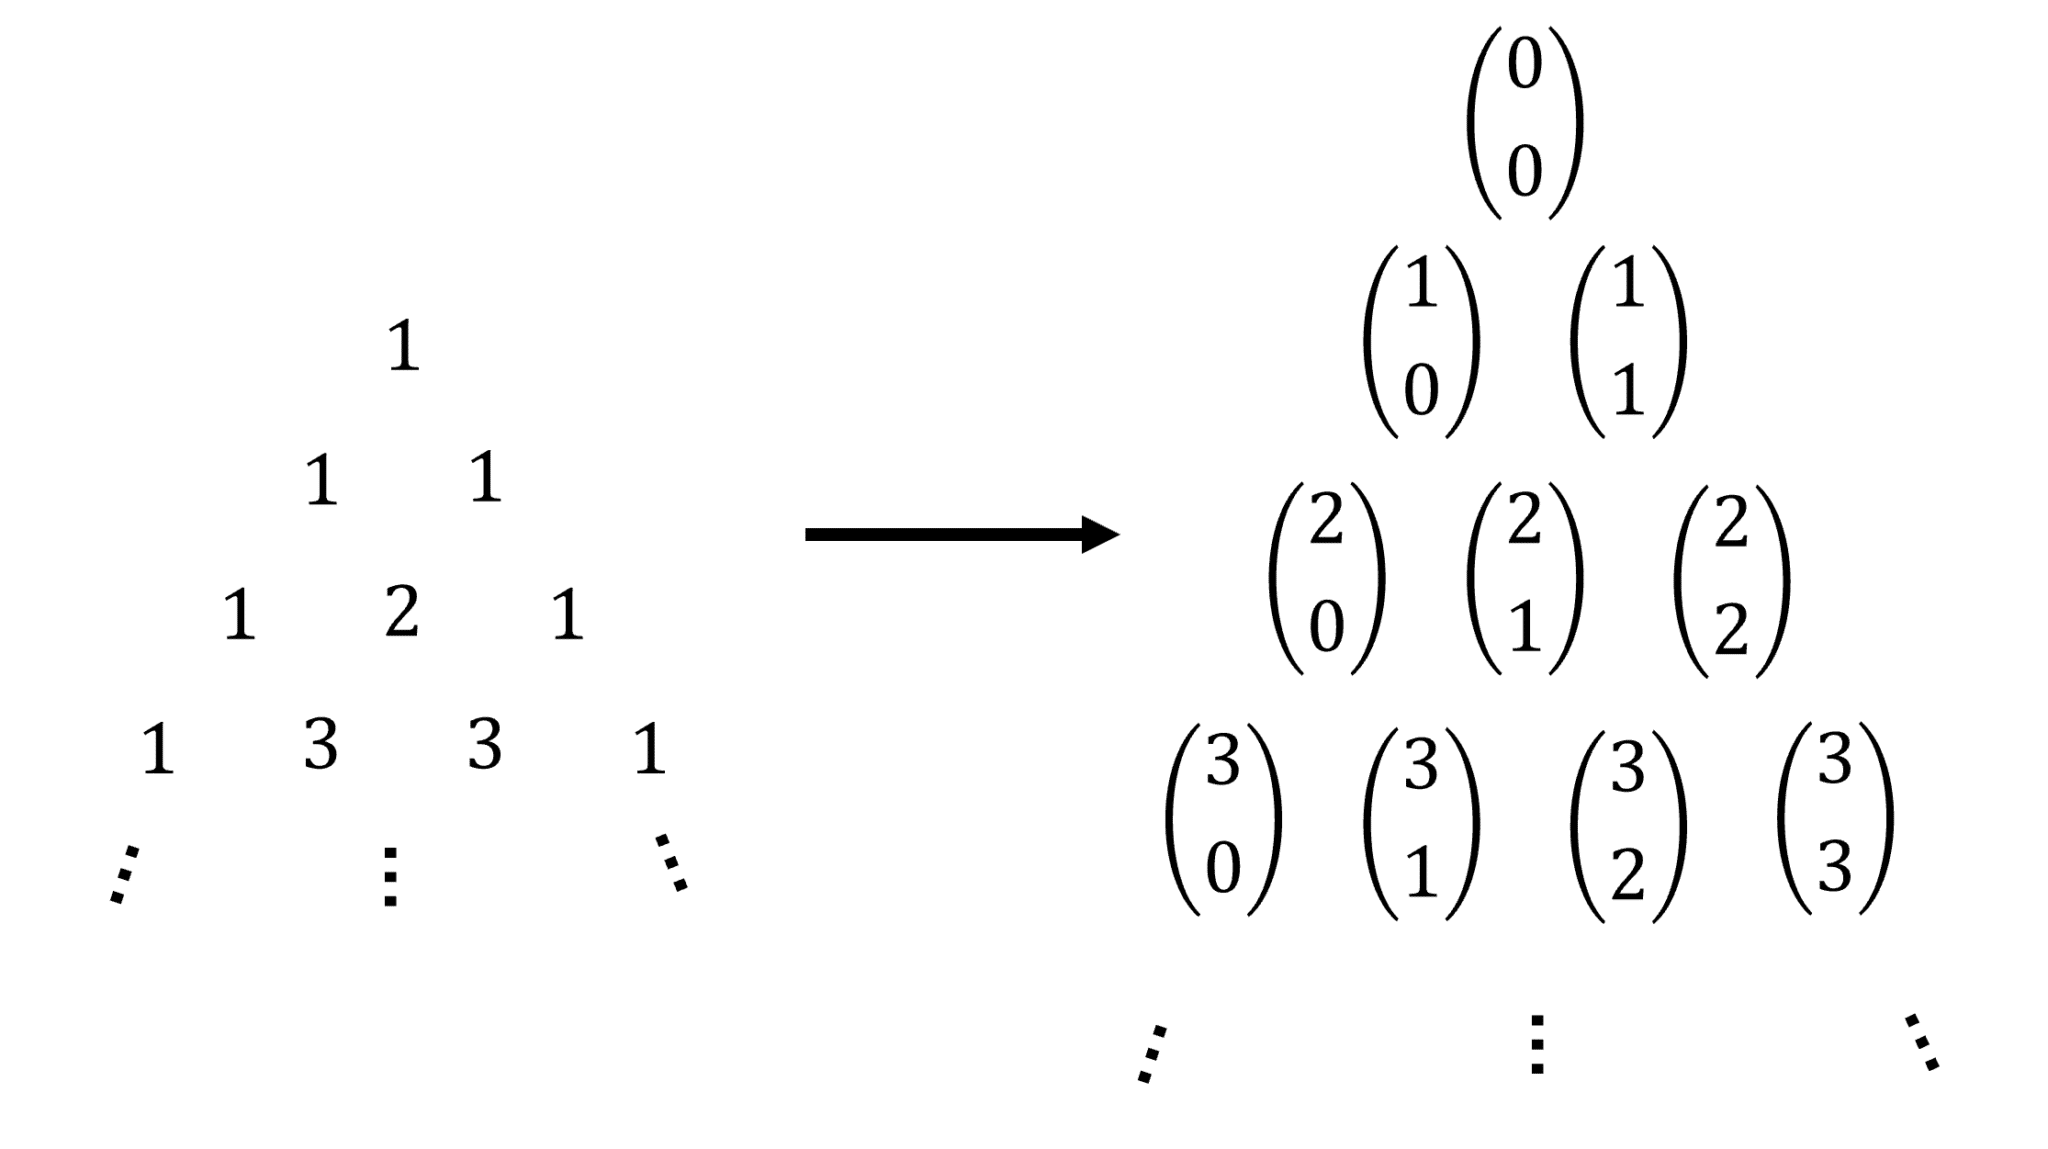
\includegraphics[width=0.5\linewidth]{imageyo.png}
    \caption{Triangle de Pascal}
    \label{fig:pascal}
\end{figure}

\begin{proposition}[Binôme de Newton]
   Soient $A$ un anneau et $a,b\in A$ tels que $ab= ba$ (ils commutent). Pour tout entier naturel $n$, on a :
   \[
   (a+b)^n = \sum_{k = 0}^n \binom{n}{k} a^k b^{n-k}
   \] 
\end{proposition}

\begin{exemple}[Équation de récurrence]
    On souhaite construire une guirlande composée de $n \ge 1$ boules. Pour ce faire, nous disposons de trois types différents de morceaux de guirlandes. Le premier est composé de deux boules bleues, le second de trois boules jaunes et le dernier de cinq boules rouges. 
    
    En notant $X_n$ le nombre de possibilités, on trouve facilement les premières valeurs : $X_1= 0$, $X_2 = 1$, $X_3=1$, $X_4=1$ et $X_5=3$. On en déduit l'équation de récurrence linéaire suivante :
    \[
  \forall n\ge 6, \quad  X_n=X_{n-2}+X_{n-3}+X_{n-5} 
    \]
    Pour la résoudre, on passe sous forme matricielle. Dès lors, on pose :
    \[
    Y_n = \begin{pmatrix}
        X_n \\ X_{n-1} \\ X_{n-2} \\ X_{n-3} \\ X_{n-4}
    \end{pmatrix}
    = \begin{pmatrix}
        0 & 1 & 1 & 0 & 1 \\
        1 & 0 & 0 & 0 & 0 \\
        0 & 1 & 0 & 0 & 0 \\
        0 & 0 & 1 & 0 & 0 \\
        0 & 0 & 0 & 1 & 0 \\
    \end{pmatrix}
    \begin{pmatrix}
        X_{n-1} \\ X_{n-2} \\ X_{n-3} \\ X_{n-4} \\ X_{n-5}
    \end{pmatrix}
    = M Y_{n-1}
    \]
    Ainsi, nous devons résoudre $Y_n = M Y_{n-1} = M^2 Y_{n-2} = \dots = M^{n-5} Y_5$. La solution générale s'écrit donc :
    \[
    Y_n = M^{n-5} Y_5 = M^{n-5} 
    \begin{pmatrix}
        3 \\ 1 \\ 1 \\ 1 \\ 0
    \end{pmatrix}
    \]
\end{exemple}

\begin{exemple}[Paradoxe des anniversaires]
    Considérons une pièce contenant $n \le 365$ personnes. Quelle est la probabilité qu'au moins deux de ces personnes aient la même date d'anniversaire ?
    
    On fait les hypothèses suivantes : l'année compte $365$ jours, et la date d'anniversaire de chaque personne est distribuée uniformément au hasard indépendamment des autres. Soit $A = [\text{au moins deux personnes partagent leur anniversaire}]$. Il est plus simple de calculer la probabilité de l'événement complémentaire $A^c = [\text{toutes les personnes ont des anniversaires différents}]$. On a :
    \begin{align*}
        P(A) &= 1 - P(A^c) \\
        &= 1 - \frac{\# A^c \text{ (cas favorables à } A^c)}{\# \Omega \text{ (tous les cas possibles)}}
    \end{align*}
    En utilisant l'analogie des urnes (on place $n$ boules discernables dans $365$ urnes), on déduit que le nombre de cas possibles sans contrainte est $365^n$. Le nombre de cas favorables à $A^c$ (au maximum une boule par urne) est $\frac{365!}{(365-n)!}$. On trouve alors :
    \[
    P(A) = 1 - \frac{365!}{365^n (365-n)!}
    \]
    Voici quelques valeurs remarquables :
    \begin{center}
    \begin{tabular}{|c|c|}
       \hline
       \textbf{Nombre de personnes} ($n$) & $\boldsymbol{P(\exists \text{ anniversaire commun})}$ \\
       \hline
       5  & $0{,}027$ \\
       15 & $0{,}253$ \\
       23 & $0{,}507$ \\
       30 & $0{,}706$ \\
       50 & $0{,}970$ \\
       70 & $0{,}999$ \\
       \hline
    \end{tabular}
    \end{center}
    \textit{Remarque : Dès 23 personnes, il y a plus de 50\,\% de chances que deux d'entre elles partagent la même date d'anniversaire.}
\end{exemple}

Cette première approche intuitive des probabilités consiste à considérer un ensemble d’événements dont on veut déterminer les chances de réalisation et y associé un nombre entre $0$ et $1$ avec l'interprétation qu'on lui a prêté plus haut. Cette approche s'avère très inintéressante pour déterminer les axiomes qui amèneront les "bonnes" propriétés intuitives qu'on espère avoir pour modéliser cette idée.


\section{Axiomatique des probabilités}



\begin{definition}
    Un \emph{espace de probabilités} est un triplet $(\Omega, \mathscr A, P)$ tel que :
    \begin{itemize}
        \item $\Omega$ est un ensemble quelconque.
        \item $\mathscr A$ est une $\sigma$-algèbre sur $\Omega$, \textit{i.e.} $\mathscr A\subseteq \partie(\Omega)$ et vérifie :
        \begin{enumerate}
            \item $\Omega\in\mathscr A$
            \item $A\in\mathscr A \alors A^c\in\mathscr A$
            \item $\displaystyle A_1,A_2,\dotsc\in\mathscr A \alors \bigcup_{n=1}^\infty A_n\in\mathscr A$
        \end{enumerate}
        \item $P$ est une mesure de probabilité, c'est-à-dire une application $P: \mathscr A \to [0,1]$ telle que :
        \begin{enumerate}
            \item $P(\Omega)=1$
            \item $P$ est $\sigma$-additive, c'est-à-dire que pour $A_1,A_2,\dots\in \mathscr A$ disjoints deux à deux ($A_i\cap A_j= \varnothing$ si $i\neq j$) :
            \[
            P\left(\bigsqcup_{n=1}^{\infty}A_n\right) = \sum_{n=1}^{\infty}P(A_n)
            \]
        \end{enumerate}
    \end{itemize}
    
    Intuitivement :
    \begin{itemize}
        \item $\Omega = \{\text{résultats possibles de l'expérience}\}$, et donc une expérience est le choix d'un $\omega\in\Omega$ (avec l'intervention du hasard).
        \item \begin{align*}
            \mathscr A &= \text{« l'ensemble des événements »}\\
            &= \text{« l'ensemble des observations que l'on sera en mesure de faire sur le résultat}\\
            &\quad \text{de l'expérience aléatoire »}
        \end{align*}
        \item \begin{align*}
            P(A) &= \text{« la mesure de probabilité de $A\in\A$ »} = \text{« la probabilité de $A$ »}\\
            &= \text{« la chance que l'événement $A$ se produise au cours de l'expérience aléatoire,}\\
            &\quad \text{ ie $\omega\in A$ »}
        \end{align*}
    \end{itemize}
\end{definition}

A présent, constatons les conséquences de cette axiomatique.

\begin{proposition}
    Soit $\mathscr A$ une $\sigma$-algèbre sur $\Omega$. Alors :
    \begin{enumerate}
        \item $\varnothing \in \mathscr A$
        \item $A_1,A_2,\dots \in \mathscr A \alors \bigcap_{n=1}^{\infty} A_n \in \mathscr A$ 
        \item $A,B\in \mathscr A \alors A\cup B\in \mathscr A,\ A\cap B \in \mathscr A,\ A\setminus B \in \mathscr A,\ A\setminus B\in \mathscr A$
    \end{enumerate}
\end{proposition}

\begin{proof}
    \begin{enumerate}
        \item $\varnothing = \Omega^c \in \A$.
        \item De $A_1,A_2,\dotsc\in\A$, on déduit $A_1^c,A_2^c,\dotsc\in\A$, d'où $\bigcup_{n=1}^\infty A_n^c\in\A$. Par les lois de De Morgan, $\bigcap_{n=1}^\infty A_n = \left(\bigcup_{n=1}^\infty A^c_n\right)^c\in\A$.
        \item Soient $A,B\in \A$. On a $A\cup B= \bigcup_{i=1}^\infty A_i$ où $A_1=A$, $A_2=B$ et $A_n= \varnothing$ si $n\ge 3$. De même, on montre que $A\cap B\in\A$. On a ensuite $A\setminus B = A\cap B^c \in \A$. Enfin, $A\setminus B = (A\setminus B)\cup (B\setminus A) \in \A$.
    \end{enumerate}
\end{proof}

Une $\sigma$-algèbre est donc un ensemble fermé par les opérations ensemblistes, ce qui est fort pratique.

\begin{proposition}
    Soit $P$ une mesure de probabilité sur $(\Omega, \A)$ :
    \begin{enumerate}
        \item $P(A\sqcup B) = P(A)+P(B)$
        \item $P(\varnothing)=0$
        \item $A,B\in \mathscr A, A\subseteq B \alors P(A) \leq P(B)$
        \item $A\in \A \alors P(A^c)= 1- P(A)$
        \item $A,B\in \A \alors P(A\cup B)= P(A)+P(B)-P(A\cap B)$
        \item $P(A\setminus B)= P(A)- P(A\cap B)$
    \end{enumerate}
\end{proposition}

\begin{proof}
    \begin{enumerate}
        \item Découle de la $\sigma$-additivité avec $A_1=A$, $A_2=B$ et $A_n=\varnothing$ pour $n \ge 3$.
        \item $P(\varnothing) = P(\varnothing \sqcup \varnothing) = P(\varnothing) + P(\varnothing) \alors P(\varnothing) = 0$.
        \item $B=A\sqcup (B\setminus A)\alors P(B)= P(A)+ P(B\setminus A)\alors P(B) \ge P(A)$ (car $P \ge 0$).
        \item $1 = P(\Omega) = P(A\sqcup A^c) = P(A)+P(A^c)$.
        \item $A\cup B= A\sqcup (B\cap A^c)\alors P(A\cup B)= P(A) + P(B\cap A^c)$. Or, $B = (B\cap A) \sqcup (B\cap A^c)$, d'où $P(B) = P(A\cap B) + P(B\cap A^c)$. En remplaçant, on obtient l'égalité voulue.
        \item $A = (A\setminus B)\sqcup(A\cap B)\alors P(A) = P(A\setminus B) + P(A\cap B)$.
    \end{enumerate}
\end{proof}

Ces propriétés sont forts naturels et souhaitable. Pour s'en rendre compte il suffit que considérer une diagramme de Venn.

\begin{exemple}[Lancer d'un dé]
    On prend $\Omega = \{1,2,3,4,5,6\}$, $\A = \partie(\Omega)$ et :
    \[
    \fonction{P}{\A\to\interff{0,1}}{A\to P(A) = \frac{\# A}{6}}
    \]
\end{exemple}

\begin{proposition}[Inégalité de Boole]
    Soient $(\Omega,\A, P)$ un espace probabiliste et $A_1,A_2,\dots \in \A$.
    \[
    P\left(\bigcup_{n=1}^{\infty}A_n\right)\leq \sum_{n=1}^\infty P(A_n)
    \]
\end{proposition}

\begin{proof}
    On définit par récurrence $B_1 = A_1$ et $B_n = A_n\setminus \bigcup_{i = 1}^{n-1}A_i$ pour $n > 1$. On a $\bigsqcup_{n=1}^\infty B_n = \bigcup_{n=1}^\infty A_n$, d'où :
    \[
    P\left(\bigcup_{n = 1}^\infty A_n\right) = P\left(\bigsqcup_{n = 1}^\infty B_n\right) = \sum_{n = 1}^\infty P(B_n) \le \sum_{n = 1}^\infty P(A_n)
    \]
    car $P(B_n)\le P(A_n)$ vu que $B_n\subseteq A_n$.
\end{proof}

\begin{proposition}[Principe d'inclusion-exclusion]
    Soient $(\Omega,\A, P)$ un espace probabiliste et $A_1,A_2,\dots, A_n \in \A$. On a :
    \[
    P\left(\bigcup_{i=1}^n A_i \right)= \sum_{k=1}^n (-1)^{k+1}\left( \sum_{1\leq i_1<\dots<i_k\leq n} P\left(\bigcap_{j=1}^k A_{i_j}\right)\right)
    \]
\end{proposition}

\begin{proof}
    La démonstration se fait par récurrence sur $n$, en utilisant l'égalité $P(A\cup B) = P(A)+P(B) - P(A\cap B)$.
\end{proof}

\section{Probabilités conditionnelles et indépendance}

\begin{definition}
    Soient $(\Omega,\A, P)$ un espace probabiliste et $A,B\in \A$ avec $P(B)\neq 0$.
    La probabilité conditionnelle de $A$ sachant $B$ est définie par :
    \[
    P(A\mid B)=\frac{P(A\cap B)}{P(B)}
    \]
    On dit que $P(A\mid B)$ est la probabilité de $A$ sachant $B$.
\end{definition}

\begin{remarque}
    Afin d'éviter d'avoir à supposer que $P(B) \neq 0$, on peut utiliser la forme multiplicative : $P(A\cap B) = P(A\mid B)P(B)$.
\end{remarque}
   
Intuitivement la probabilité de $A$ sachant $B$ est la probabilité que la "fraction" de $A$ qui se réalise lorsque $B$ est réalisé.

\begin{exemple}[Lancer d'un dé]
    $A=[\text{le résultat est 4}]$, $B=[\text{le résultat est pair}]$. 
    Ici, $P(A\mid B)= \frac{P(A\cap B)}{P(B)} = \frac{P(A)}{P(B)}= \frac{1/6}{1/2} = \frac{1}{3}$.
\end{exemple}

\begin{remarque}
    L'application 
    \[
    \fonction{P_B}{\A}{\interff{0}{1}}{A}{P_B(A) = P(A\mid B)}
    \]
    est une mesure de probabilité. Toutes les propriétés des mesures de probabilité restent donc vraies pour $P_B$.
\end{remarque}

\begin{exercice}[Événement certain]
    Montrer que si $P(A)=1$, alors pour tout événement $B$ tel que $P(B)>0$, on a $P(A\mid B)=1$.
\end{exercice}

\begin{theoreme}[Probabilités totales]
    Soient $(\Omega,\A, P)$ un espace probabiliste et $\{B_n\}$ une partition finie ou dénombrable de $\Omega$ vérifiant $\forall n,\ B_n\in \A$ et $P(B_n)>0$. Alors :
    \[
    P(A) = \sum_n P(A\mid B_n)P(B_n)
    \]
\end{theoreme}

\begin{proof}
    Nous avons que :
    \begin{align*}
        P(A) &= P(A\cap \Omega)\\
        &= P\left(A\cap \left(\bigsqcup_n B_n\right)\right)\\ 
        &= \sum_{n} P(A\cap B_n)\\ 
        &= \sum_n P(A\mid B_n)P(B_n)
    \end{align*}  
\end{proof}



\begin{exemple}
    Supposons qu'il n'y ait que deux temps possibles demain :
    \begin{itemize}
        \item Pas beau : $20\%$ de chances que je sorte.
        \item Beau : $70\%$ de chances que je sorte.
    \end{itemize}
    Quelle est la probabilité que je sorte demain, sachant que la météo m'informe qu'il y a $40\%$ de chances de mauvais temps ?
    \[
    P(\text{sors}) = P(\text{sors}\mid \text{beau})P(\text{beau}) + P(\text{sors}\mid \text{pas beau})P(\text{pas beau}) = 0{,}7\cdot 0{,}6 + 0{,}2\cdot 0{,}4 = 0{,}5
    \]
\end{exemple}

\begin{proposition}[Règle de Bayes]
    Soient $(\Omega,\A, P)$ un espace probabiliste et $A,B\in \A$ avec $P(B)\neq 0$. Nous avons que :
    \[
    P(A\mid B)= \frac{P(B\mid A)P(A)}{P(B)}
    \]
\end{proposition}

\begin{proof}
    Nous avons que :
    \begin{align*}
       P(A\mid B) &= \frac{P(A\cap B)}{P(B)} \\
       &= \frac{P(B\cap A)}{P(B)} \\
       &= \frac{P(B\mid A)P(A)}{P(B)}
    \end{align*}   
\end{proof}

\begin{exemple}[Paradoxe du faux positif]
    Une infection mortelle (le covid-10000) se propage dans une population, et on dispose d'un test PCR. Le vendeur nous indique que :
    \begin{itemize}
        \item Il y a $95\%$ de chances que le test soit positif si la personne testée est infectée.
        \item Il y a $1\%$ de chances de faux positifs (test positif alors que la personne est saine).
        \item $0{,}5\%$ de la population est infectée.
    \end{itemize}
    De plus, un traitement existe, mais il est très risqué ($50\%$ de chances d'être mortel). Si une personne se présente avec un test positif, doit-elle prendre le traitement ?
\end{exemple}

\begin{proof}[Résolution]
    Posons $A = [\text{l'individu est infecté}]$ et $B=[\text{le test est positif}]$. 
    \begin{align*}
        P(A\mid B) &= \frac{P(B\mid A)P(A)}{P(B)}\\ 
        &= \frac{P(B\mid A)P(A)}{P(B\mid A)P(A)+P(B\mid A^c)P(A^c)}\\
        &= \frac{0{,}95\cdot 0{,}005}{0{,}95\cdot 0{,}005 + 0{,}01\cdot 0{,}995} \simeq 0{,}323
    \end{align*}
    La probabilité d'être réellement malade sachant que le test est positif n'est que d'environ $32{,}3\%$. Prendre un traitement mortel dans $50\%$ des cas serait donc déraisonnable. Il y a ici une confusion classique entre $P(A\mid B)$ et $P(B\mid A)$.
\end{proof}

\begin{notation}
    On note souvent $P(A,B)= P(A\cap B)$ et $P(A\mid B,C)= P(A\mid B\cap C)$.
\end{notation}

\begin{definition}[Indépendance]
    Soient $(\Omega, \A,P)$ un espace de probabilités et $A,B\in\A$. On dit que $A$ et $B$ sont indépendants, ce que l'on note $A\indep B$, si $P(A\cap B) = P(A)P(B)$, ou, de façon équivalente (si $P(B)>0$), si $P(A \mid B) = P(A)$.
\end{definition}

\begin{exemple}[Lancer de $2$ pièces]
    On note $A=[\text{la pièce } 1 \text{ tombe sur pile}]$, $B= [\text{la pièce } 2 \text{ tombe sur pile}]$ et $C=[\text{les deux pièces tombent sur pile}]$.
    \begin{itemize}
        \item $A\indep B$ : On a $P(A\cap B) =\frac{1}{4} = \frac{1}{2}\cdot\frac{1}{2} = P(A)P(B)$.
        \item $A\nindep C$ : On a $P(A\cap C) = P(C) = \frac{1}{4}$ mais $P(A)P(C) = \frac{1}{2}\cdot\frac{1}{4} = \frac{1}{8}$.
    \end{itemize}
\end{exemple}

\begin{definition}
    Soient $(\Omega, \A,P)$ un espace de probabilités et $(A_i)_{i\in I}$ une famille d'événements.
    \begin{itemize}
        \item Les $A_i$ sont \emph{indépendants deux à deux} si :
        \[
        \forall i\neq j, \quad A_i \indep A_j 
        \]
        \item Les $A_i$ sont \emph{mutuellement indépendants} (ou indépendants dans leur ensemble) si :
        \[
        \forall J\subseteq I \text{ fini}, \quad P\left(\bigcap_{j\in J}A_j\right)=\prod_{j\in J}P(A_j)
        \]
    \end{itemize}
\end{definition}

\begin{exemple}
    On a $4$ cartes : rouge, verte, bleue et multicolore (contenant les 3 couleurs). On tire une carte au hasard, et on pose $R = [\text{la carte contient du rouge}]$ ; de même pour $B$ et $V$.
    \begin{description}
        \item[$R, B, V$ sont indépendants deux à deux :] On a $P(R\cap B) = \frac{1}{4}$ (seule la carte multicolore contient à la fois du rouge et du bleu). Or, $P(R) = P(B) = P(V) = \frac{2}{4} = \frac{1}{2}$. On a bien $P(R\cap B) = P(R)P(B) = \frac{1}{4}$.
        \item[$R, B, V$ ne sont pas mutuellement indépendants :] On a $P(R\cap B\cap V) = \frac{1}{4}$ (la carte multicolore), ce qui est différent de $P(R)P(B)P(V) = \frac{1}{8}$.
    \end{description}
\end{exemple}

\begin{exemple}[Affaire Sally Clark]
    \begin{itemize}
        \item Il y a environ $0{,}01\%$ de chances qu'un nourrisson meure de mort subite.
        \item L'expert a calculé les chances que les deux enfants meurent de mort subite ainsi : $\frac{1}{10^4} \cdot \frac{1}{10^4} = \frac{1}{10^8} \simeq 0$.
    \end{itemize}
    Ce raisonnement souffre de deux problèmes majeurs :
    \begin{itemize}
        \item L'hypothèse d'indépendance (la génétique ou l'environnement rendent ces événements dépendants).
        \item Il y a eu une confusion entre deux probabilités conditionnelles (le sophisme du procureur). Posons $I = [\text{Sally est innocente}]$ et $M = [\text{les deux enfants meurent en bas âge}]$. L'argument de l'expert porte sur $P(M\mid I)$, or ce qui intéresse la justice est $P(I\mid M)$. Par la formule de Bayes :
        \[
        P(I\mid M ) = \frac{P(M\mid I)P(I)}{P(M\mid I)P(I) + P(M\mid I^c)P(I^c)} \simeq 1
        \]
        vu que $P(I^c)$ (la probabilité a priori qu'une mère soit une double meurtrière) est extrêmement faible, proche de $0$.
    \end{itemize}
\end{exemple}

\section{Suites d'événements, lemme de Borel-Cantelli}

\begin{definition}
    Soient $(\Omega, \A, P)$ un espace de probabilité et $(A_n)$ une suite d'événements dans $\A$.
    \begin{itemize}
        \item Si $(A_n)$ est croissante, ie $(A_n \subseteq A_{n+1})$, on définit sa limite comme :
        \[
        \lim_{n\to +\infty}A_n = \bigcup_{n=1}^{\infty} A_n
        \]
        \item Si $(A_n)$ est décroissante, ie $(A_{n+1} \subseteq A_n)$, on définit sa limite comme :
        \[
        \lim_{n\to +\infty}A_n = \bigcap_{n=1}^{\infty} A_n
        \]
    \end{itemize}
\end{definition}

\begin{theoreme}[Continuité des probabilités]
    Si $(A_n)$ est une suite monotone dans $\A$, alors :
    \[
    \lim_{n\to\infty} P(A_n) = P\left(\lim_{n\to\infty}A_n\right)
    \]
\end{theoreme}

\begin{proof}
    \textbf{Cas où $(A_n)$ est croissante :} On pose $B_1 = A_1$ et $B_k = A_k\setminus A_{k-1}$ pour $k \ge 2$. Les ensembles $B_k$ sont disjoints et on a :
    \[
    \bigsqcup_{n=1}^\infty B_n = \bigcup_{n=1}^\infty A_n
    \]
    Par la $\sigma$-additivité de $P$, on obtient :
    \begin{align*}
        P\left( \bigcup_{n=1}^{\infty}A_n\right) &= P\left(\bigsqcup_{n=1}^{\infty}B_n\right)\\
        &= \sum_{n = 1}^\infty P(B_n) = \lim_{N\to\infty} \sum_{n = 1}^N P(B_n)\\
        &= \lim_{N\to\infty} P\left(\bigsqcup_{n = 1}^N B_n\right) = \lim_{N\to\infty}P(A_N)
    \end{align*}
    
    \textbf{Cas où $(A_n)$ est décroissante :} On considère la suite complémentaire $(A^c_n)$, qui est croissante. Par les lois de De Morgan et le point précédent :
    \[
    P\left(\bigcap_{n=1}^\infty A_n\right) = 1 - P\left(\bigcup_{n=1}^\infty A^c_n\right) = 1 - \lim_{N\to\infty}P(A^c_N) = \lim_{N\to\infty} P(A_N)
    \]
\end{proof} 

\begin{exercice}[L'urne de minuit]
    Nous possédons une urne de capacité infinie. À minuit moins une minute, on place $10$ boules numérotées de $1$ à $10$ dans l'urne et on retire la boule n°10. À minuit moins 30 secondes, on place $10$ boules numérotées de $11$ à $20$ et on retire la boule n°20, et ainsi de suite jusqu'à minuit. On constate qu'à minuit, il y a un nombre infini de boules dans l'urne. 
    
    Modifions un peu les règles : à l'étape $n$, au lieu de retirer systématiquement la boule ayant le plus grand numéro, \textbf{on tire une boule uniformément au hasard} parmi toutes les boules présentes dans l'urne. Combien de boules reste-t-il dans l'urne à minuit ?
    
    \textit{Contre toute attente, avec cette modification, à minuit l'urne est presque sûrement vide !}
    
    \medskip\noindent \textbf{Résolution :} 
    Notons $A_1=[\text{la boule n°1 est dans l'urne à minuit}]$ et $A_1^{(n)}= [\text{la boule n°1 est présente à l'étape } n]$.
    À l'étape $n$, il y a $9n+1$ boules dans l'urne juste avant le retrait. La probabilité que la boule n°1 \textbf{ne soit pas} tirée à cette étape est donc $\frac{9n}{9n+1}$.
    On a :
    \[
    P(A_1) = P\left(\bigcap_{n=1}^\infty A_1^{(n)}\right) = \lim_{N\to\infty} P\left(A^{(N)}_1\right) = \prod_{n = 1}^\infty \frac{9n}{9n+1} = 0.
    \]
    On peut faire le même raisonnement pour n'importe quelle boule n°$i$ : $P(A_i) = 0$. Donc, par l'inégalité de Boole :
    \begin{align*}
        P(\text{l'urne est non vide à minuit}) &= P\left(\bigcup_{i = 1}^\infty A_i\right) \le \sum_{i = 1}^\infty P(A_i) = 0
    \end{align*}
\end{exercice}

\begin{proof}[Détail : Montrons que le produit vaut bien $0$]
    Pour montrer qu'un produit de probabilités tend vers $0$, on étudie souvent son inverse. On a :
    \begin{align*}
        \prod_{n = 1}^\infty \frac{9n + 1}{9n} = \prod_{n = 1}^\infty \left(1 + \frac{1}{9n}\right) \ge \sum_{n = 1}^\infty \frac{1}{9n} = +\infty  
    \end{align*}
    Puisque le produit inverse diverge vers l'infini (série harmonique), le produit initial converge bien vers $0$.
\end{proof}

\begin{proposition}
    Soit $(\Omega, \A, P)$ un espace probabiliste et $(A_n)$ une suite d'événements dans $\A$. On pose :
    \[
    \limsup_{n\to+\infty} A_n = \bigcap_{n=1}^\infty \bigcup_{k = n}^\infty A_k \qquad \text{et} \qquad \liminf_{n\to+\infty} A_n = \bigcup_{n=1}^\infty \bigcap_{k = n}^\infty A_k
    \]
    Si $\limsup_{n\to +\infty}A_n = \liminf_{n\to +\infty}A_n = A$, alors on dit que la limite de la suite $(A_n)$ existe et on note $\lim_{n\to +\infty}A_n = A$.
\end{proposition}

\begin{proof}
   Intuitivement, ces ensembles ont une signification probabiliste forte :
    \[
    \bigcup_{k=m}^{\infty} A_k = \{\omega \in \Omega \mid \exists k \geq m : \omega \in A_k\}
    \]
    Donc :
    \[
    \limsup_{n \to +\infty} A_n = \{\omega \in \Omega \mid \forall m,\ \exists k \geq m : \omega \in A_k\} = [A_n \text{ infiniment souvent (i.s.)}]
    \]
    Cela signifie que l'événement se produit une infinité de fois.
    
    De même pour la limite inférieure :
    \[
    \liminf_{n \to +\infty} A_n = \bigcup_{m=1}^{\infty} \bigcap_{k=m}^{\infty} A_k = \{\omega \in \Omega \mid \exists m,\ \forall k \geq m : \omega \in A_k\} = [A_n \text{ ultimement (e.o.)}]
    \]
    Cela signifie que l'événement se produit à chaque fois, à partir d'un certain rang (ou avec un nombre fini d'exceptions, \textit{eventually occurring}).
\end{proof}

\begin{theoreme}[Lemme de Borel-Cantelli]
    Soit $(\Omega, \A, P)$ un espace probabiliste et $(A_n)$ une suite d'événements.
\begin{enumerate}
    \item Si $\displaystyle\sum_{n=1}^{\infty} P(A_n) < \infty$, alors $P\left(\limsup_{n \to +\infty} A_n\right) = 0$.
    \item Si $\displaystyle\sum_{n=1}^{\infty} P(A_n) = \infty$ \textbf{et que les $A_n$ sont indépendants}, alors $P\left(\limsup_{n \to +\infty} A_n\right) = 1$.
\end{enumerate}
\end{theoreme}

\begin{proof}
    \textbf{Preuve de la partie 1 :}
    \[
    P\left(\limsup_{n \to +\infty} A_n\right) = P\left(\bigcap_{m=1}^{\infty}\bigcup_{k=m}^{\infty} A_k\right) \leq P\left(\bigcup_{k=m}^{\infty} A_k\right) \quad \forall m
    \]
    Par l'inégalité de Boole :
    \[
    P\left(\limsup_{n \to +\infty} A_n\right) \leq \sum_{k=m}^{\infty} P(A_k) \quad \forall m 
    \]
    En passant à la limite quand $m \to +\infty$, on évalue le reste d'une série convergente, qui tend vers $0$ :
    \[
    \implies P\left(\limsup_{n \to +\infty} A_n\right) \leq \lim_{m \to +\infty} \sum_{k=m}^{\infty} P(A_k) = 0
    \]
    
    \textbf{Preuve de la partie 2 :}
    \begin{align*}
    P\left(\limsup_{n \to +\infty} A_n\right)
    &= 1 - P\left(\left(\limsup_{n \to +\infty} A_n\right)^c\right) \\
    &= 1 - P\left(\left(\bigcap_{m=1}^{\infty}\bigcup_{k=m}^{\infty} A_k\right)^c\right) \\
    &= 1 - P\left(\bigcup_{m=1}^{\infty}\bigcap_{k=m}^{\infty} A_k^c\right) \\
    &= 1 - \lim_{m \to +\infty} P\left(\bigcap_{k=m}^{\infty} A_k^c\right) \qquad (\text{Car la suite d'intersections est croissante en } m) \\
    &= 1 - \lim_{m \to +\infty} \lim_{N \to +\infty} P\left(\bigcap_{k=m}^{N} A_k^c\right) \qquad (\text{Continuité des probabilités}) \\
    &= 1 - \lim_{m \to +\infty} \lim_{N \to +\infty} \prod_{k=m}^{N} P(A_k^c) \qquad (\text{Car les } A_k \text{ sont indépendants}) \\
    &= 1 - \lim_{m \to +\infty} \lim_{N \to +\infty} \prod_{k=m}^{N} \bigl(1 - P(A_k)\bigr) \\
    &\leq 1 - \lim_{m \to +\infty} \lim_{N \to +\infty} \prod_{k=m}^{N} e^{-P(A_k)} \qquad (\text{Utilisation de } 1-x \leq e^{-x}) \\
    &= 1 - \lim_{m \to +\infty} \lim_{N \to +\infty} e^{-\sum_{k=m}^{N} P(A_k)} \\
    &= 1 - 0 \qquad (\text{Car la série } \textstyle\sum P(A_k) \text{ diverge vers l'infini}) \\
    &= 1
    \end{align*}
\end{proof}

\begin{remarque}
\begin{itemize}
    \item Le lemme de Borel-Cantelli est un des théorèmes fondateurs des « lois du 0-1 » en probabilités : l'événement limite se produit soit avec une probabilité de $0$, soit de $1$.
    \item Est-ce que $P\left(\limsup_{n\to+\infty} A_n\right) = \limsup_{n\to+\infty} P(A_n)$ ? \textcolor{PropColor}{\textbf{Non}}, la continuité des probabilités ne s'applique qu'aux suites monotones. Borel-Cantelli permet justement de contourner ce problème.
\end{itemize}
\end{remarque}

\begin{exemple}[Série convergente : Les pièces truquées]
    On joue à pile ou face à répétition. Les pièces sont truquées et se fatiguent avec le temps :
    \[
    \text{Lors de la partie } n : \quad P(\text{face}) = \frac{1}{n^2}
    \]
    Est-ce qu'on obtiendra une infinité de « face » au cours du jeu ?
    
    Posons $A_n = [\text{on obtient face au } n^\text{e} \text{ lancer}]$. Alors :
    \[
    \sum_{n=1}^{\infty} P(A_n) = \sum_{n=1}^{\infty} \frac{1}{n^2} < \infty \quad \text{(série de Riemann convergente)}
    \]
    Par la première partie du lemme de Borel-Cantelli :
    \[
    P(A_n \text{ i.s.}) = 0
    \]
    \textbf{Conclusion :} À partir d'un certain moment (qui dépend de l'expérience), on n'obtiendra plus jamais de face ! Le résultat « face » s'arrête presque sûrement.
\end{exemple}

\begin{exemple}[Série divergente : Le paradoxe du singe savant]
    \og Un singe immortel, tapant au hasard sur un clavier, finira par écrire l'œuvre complète de Shakespeare. Il l'écrira même une infinité de fois. \fg{}
    
    \medskip
    \noindent \textbf{Formalisation et Résolution :}
    \begin{itemize}
        \item $\mathcal{L}$ est l'ensemble des caractères du clavier, de taille constante $\#\mathcal{L} = L$.
        \item $S_H$ est le texte de Shakespeare, qui est une suite précise de longueur fixe $n$.
        \item On découpe le temps de frappe du singe en blocs disjoints de taille $n$.
    \end{itemize}
    Posons $A_m = [\text{le texte } S_H \text{ est écrit exactement dans le } m^\text{e} \text{ bloc (entre les frappes } mn \text{ et } mn+n)]$. 
    
    Si on regardait chaque lettre une par une (des blocs superposés), les événements ne seraient pas indépendants. Mais en prenant des blocs disjoints ($A_1, A_2, A_3, \dots$), les événements deviennent \textbf{indépendants}.
    
    La probabilité de taper le bon texte sur un bloc donné est $P(A_m) = \left(\frac{1}{L}\right)^n$. \textbf{Attention : $n$ est fixe !} Cette probabilité est donc une constante $c > 0$. On a alors :
    \[
    \sum_{m=1}^{\infty} P(A_m) = \sum_{m=1}^{\infty} \left(\frac{1}{L}\right)^n = \sum_{m=1}^{\infty} c = +\infty
    \]
    Puisque la somme diverge et que les événements sont indépendants, la deuxième partie du lemme de Borel-Cantelli s'applique : $P(A_m \text{ i.s.}) = 1$. Le singe réécrira le texte une infinité de fois.
\end{exemple}

\begin{exemple}[Marche aléatoire dans $\mathbb{Z}$ avec $p \neq \frac{1}{2}$]
    Imaginons un homme ivre marchant sur une ligne. À chaque pas, il va à droite avec une probabilité $p$ ou à gauche avec une probabilité $(1-p)$. Si $p \neq 1/2$, le jeu est asymétrique. L'état de départ $0$ va-t-il être visité une infinité de fois ?
    
    Posons $A_n = [\text{l'homme est à l'origine au temps } n]$.
    Pour revenir en $0$, il faut avoir fait autant de pas à droite qu'à gauche. C'est impossible en un nombre impair de pas, donc $P(A_{2n-1}) = 0$.
    Pour un nombre pair de pas ($2n$), il faut exactement $n$ pas à droite et $n$ pas à gauche :
    \[
    P(A_{2n}) = \binom{2n}{n} p^n (1-p)^n
    \]
   Par conséquent :
    \[
    \sum_{n=1}^{\infty} P(A_{2n}) < \infty
    \]
    Par le lemme de Borel-Cantelli, $P(A_n \text{ i.s.}) = 0$. \textbf{Conclusion :} Un marcheur asymétrique finira par s'éloigner pour toujours et ne reviendra plus jamais à son point de départ.
\end{exemple}
\chapter{Variables aléatoires}

\section{Variables aléatoires et leur loi}

Jusqu'à présent, nous avons décrit une expérience aléatoire de manière abstraite via un espace de probabilités $(\Omega, \A, P)$. En pratique, on s'intéresse rarement au résultat brut $\omega \in \Omega$ de l'expérience, mais plutôt à une grandeur numérique déduite de ce résultat (un gain à un jeu, le temps d'attente avant une panne, la somme de deux dés, etc.). 

On modélise cette quantité d'intérêt par une fonction $X$ qui, à chaque issue possible $\omega$, associe un nombre réel :
\[
X : \Omega \longrightarrow \R
\]

\begin{definition}[Variable aléatoire]
    Une \emph{variable aléatoire} (souvent abrégée en v.a.) sur un espace probabilisé $(\Omega, \A, P)$ est une application
    \[
    X : \Omega \longrightarrow \R
    \]
    qui est \emph{mesurable}, c'est-à-dire qui vérifie :
    \[
    \forall U \in \mathcal{B}(\R), \quad X^{-1}(U) \in \A
    \]
    où $\mathcal{B}(\R)$ est la tribu borélienne sur $\R$ (la plus petite $\sigma$-algèbre contenant tous les ouverts de $\R$).
\end{definition}

\begin{remarque}
    La condition de mesurabilité sert de « filet de sécurité ». Elle garantit que pour n'importe quel ensemble de valeurs $U$ (par exemple un intervalle de $\R$), l'ensemble des issues originelles qui conduisent à ce résultat  noté $X^{-1}(U) = \{\omega \in \Omega \mid X(\omega) \in U\}$  est bien un événement de $\A$. On peut donc lui attribuer une probabilité.
\end{remarque}

\begin{notation}
    Pour alléger l'écriture, au lieu d'écrire la probabilité de l'événement originel $P(\{\omega \in \Omega \mid X(\omega) \in U\})$, on notera simplement :
    \[
    P(X \in U) = P\!\left(X^{-1}(U)\right)
    \]
\end{notation}

\begin{exemple}[Lancer de deux dés]
    On lance deux dés à six faces parfaits. Le modèle naturel est :
    \begin{itemize}
        \item L'univers $\Omega = \{(i,j) \mid i,j \in \{1,\dotsc,6\}\}$ (les 36 couples de résultats possibles).
        \item La tribu $\A = \partie(\Omega)$.
        \item La probabilité uniforme $P(A) = \frac{\#A}{36}$.
    \end{itemize}
    On s'intéresse à la variable aléatoire $X$ représentant la \textbf{somme des deux dés}. Formellement :
    \[
    \fonction{X}{\Omega\to\R}{(\omega_1, \omega_2) \to \omega_1 + \omega_2}
    \]
    Quelle est la probabilité d'obtenir une somme égale à 5 ?
    \begin{align*}
        P(X = 5) &= P\!\left(X^{-1}(\{5\})\right) \\
        &= P\!\left(\{(1,4), (4,1), (2,3), (3,2)\}\right) \\
        &= \frac{4}{36} = \frac{1}{9}
    \end{align*}
\end{exemple}

\begin{definition}[Loi d'une variable aléatoire]
    Soit $X$ une variable aléatoire sur $(\Omega, \A, P)$. L'application $P_X : \mathcal{B}(\R) \longrightarrow [0,1]$ définie par :
    \[
    P_X(U) = P\!\left(X^{-1}(U)\right) = P(X \in U)
    \]
    est une mesure de probabilité sur l'espace mesurable $(\R, \mathcal{B}(\R))$. On l'appelle la \emph{loi de la variable aléatoire} $X$.
\end{definition}

L'intérêt majeur de la loi $P_X$ est qu'elle contient \textbf{toute l'information probabiliste} concernant la variable $X$.

\begin{definition}[Égalité en loi]
    Soient $X$ et $Y$ deux variables aléatoires (éventuellement définies sur des espaces de probabilité différents). Si elles ont la même loi, c'est-à-dire si $P_X = P_Y$, on dit qu'elles sont \emph{égales en loi} et on note :
    \[
    X \overset{d}{=} Y \quad \text{ou} \quad X \sim Y
    \]
    D'un point de vue probabiliste, deux variables égales en loi sont indiscernables, même si elles décrivent des phénomènes physiques totalement différents.
\end{definition}

\begin{exemple}[Deux variables de même loi sur des espaces différents]
    Cet exemple illustre parfaitement le concept d'égalité en loi.
    
    \textbf{Expérience 1 :} On lance deux pièces de monnaie équilibrées. 
    \begin{itemize}
        \item $\Omega_1 = \{(P,P), (P,F), (F,P), (F,F)\}$. Probabilité uniforme ($1/4$ chaque).
        \item On définit $X =$ « le nombre de piles obtenus ».
        \item Les valeurs de $X$ sont $X(P,P) = 2$, $X(P,F) = 1$, $X(F,P) = 1$, $X(F,F) = 0$.
    \end{itemize}
    La loi de $X$ (notée $P_X$) est donnée par :
    \[
    P(X=0) = \frac{1}{4}, \quad P(X=1) = \frac{2}{4} = \frac{1}{2}, \quad P(X=2) = \frac{1}{4}
    \]

    \textbf{Expérience 2 :} On tire un numéro au hasard dans une urne contenant 4 boules numérotées $\{1, 2, 3, 4\}$.
    \begin{itemize}
        \item $\Omega_2 = \{1, 2, 3, 4\}$. Probabilité uniforme ($1/4$ chaque).
        \item On définit la variable $Y : \Omega_2 \to \R$ par le tableau de valeurs suivant :
        $Y(1) = 0$, $Y(2) = 1$, $Y(3) = 1$, $Y(4) = 2$.
    \end{itemize}
    La loi de $Y$ (notée $P_Y$) est donnée par :
    \[
    P(Y=0) = \frac{1}{4}, \quad P(Y=1) = \frac{2}{4} = \frac{1}{2}, \quad P(Y=2) = \frac{1}{4}
    \]
    
     Bien que modélisant des situations très différentes (des pièces de monnaie contre des boules numérotées) et ayant des univers différents ($\Omega_1 \neq \Omega_2$), les lois coïncident parfaitement ($P_X = P_Y$). On a donc $X \overset{d}{=} Y$.
\end{exemple}

\begin{definition}[Fonction de répartition]
    Soit $X$ une variable aléatoire sur $(\Omega, \A, P)$. La \emph{fonction de répartition} de $X$ est la fonction $F_X: \R \to [0,1]$ définie par :
    \begin{align*}
       F_X(x) &= P(X \leq x) \\
       &= P_X(]-\infty, x]) \\
       &= P\!\left(X^{-1}(]-\infty, x])\right)
    \end{align*}
\end{definition}

\begin{remarque}
    Tout comme la loi $P_X$, la fonction de répartition caractérise entièrement la variable aléatoire. Connaître $F_X$, c'est connaître la loi de $X$.
\end{remarque}

\begin{proposition}[Propriétés de la fonction de répartition]
    La fonction de répartition $F_X$ d'une variable aléatoire vérifie toujours les trois propriétés fondamentales suivantes :
    \begin{enumerate}
        \item $F_X$ est croissante sur $\R$.
        \item Les limites aux bornes sont : $\displaystyle\lim_{x\to -\infty} F_X(x)=0 \quad \text{et} \quad \lim_{x\to +\infty} F_X(x)=1$.
        \item $F_X$ est continue à droite en tout point : $\displaystyle\lim_{x \searrow a} F_X(x) = F_X(a)$.
    \end{enumerate}
\end{proposition}

\begin{proof}
    Ces propriétés découlent directement des axiomes des probabilités :
    \begin{description}
        \item[(1) Croissance :] Soient $x, y \in \R$ tels que $x \leq y$. Alors $]-\infty, x] \subseteq ]-\infty, y]$. Par monotonie de la mesure de probabilité, on a $P(X \leq x) \leq P(X \leq y)$, ce qui signifie exactement $F_X(x) \leq F_X(y)$.
        
        \item[(2) Limites aux bornes :] Considérons une suite croissante $(x_n)$ qui tend vers $+\infty$. La suite d'événements $A_n = \{X \leq x_n\}$ est croissante et son union vaut $\Omega$ (car $X$ prend des valeurs réelles finies). Par continuité croissante des probabilités :
        \[
        \lim_{n\to \infty} F_X(x_n) = \lim_{n\to \infty} P(A_n) = P\left(\bigcup_{n=1}^\infty A_n\right) = P(\Omega) = 1
        \]
        De même, si $(x_n)$ décroît vers $-\infty$, l'intersection des événements $\{X \leq x_n\}$ est vide. Par continuité décroissante, la limite vaut $P(\varnothing) = 0$.
        
        \item[(3) Continuité à droite :] Soit $a \in \R$ et une suite $(x_n)$ décroissant strictement vers $a$ ($x_n \searrow a$). La suite d'événements $B_n = \{X \leq x_n\}$ est décroissante et son intersection est l'événement $\{X \leq a\}$. Par continuité décroissante :
        \[
        \lim_{n\to \infty} F_X(x_n) = \lim_{n\to \infty} P(B_n) = P\left(\bigcap_{n=1}^\infty B_n\right) = P(X \leq a) = F_X(a)
        \]
    \end{description}
\end{proof}

\newpage

\begin{proposition}[Calculs avec la fonction de répartition]
    Pour tous réels $a < b$, nous avons :
    \begin{enumerate}
        \item $P(a < X \leq b) = F_X(b) - F_X(a)$
        \item $P(X < a) = \displaystyle\lim_{x \nearrow a} F_X(x) = F_X(a^-)$ (limite à gauche)
    \end{enumerate}
\end{proposition}

\begin{proof}
    \begin{description}
        \item[(1)] On peut écrire l'événement $\{X \leq b\}$ comme une union disjointe :
        \[
        \{X \leq b\} = \{X \leq a\} \sqcup \{a < X \leq b\}
        \]
        Par additivité de la probabilité, on obtient :
        \[
        P(X \leq b) = P(X \leq a) + P(a < X \leq b)
        \]
        Ce qui donne directement $F_X(b) = F_X(a) + P(a < X \leq b)$.
        
        \item[(2)] Considérons une suite $(a_n)$ croissant strictement vers $a$ ($a_n \nearrow a$). La suite d'événements $\{X \leq a_n\}$ est croissante, et son union (strictement avant d'atteindre $a$) est l'événement ouvert $\{X < a\}$. Par continuité des probabilités :
        \[
        P(X < a) = P\left(\bigcup_{n=1}^\infty \{X \leq a_n\}\right) = \lim_{n\to \infty} P(X \leq a_n) = \lim_{n\to \infty} F_X(a_n) = \lim_{x \nearrow a} F_X(x)
        \]
    \end{description} 
\end{proof}

\section{Variables aléatoires discrètes}

\subsection{Définitions fondamentales}

\begin{definition}[Variable aléatoire discrète]
    Une variable aléatoire $X$ sur un espace probabilisé $(\Omega, \A, P)$ est dite \emph{discrète} si elle ne prend qu'un nombre fini ou au plus dénombrable de valeurs $\{x_1, x_2, \dots, x_n, \dots\}$.
\end{definition}

\begin{definition}[Fonction de masse]
    La \emph{fonction de masse} (souvent appelée distribution de probabilité) de la variable discrète $X$ est l'ensemble des probabilités associées à chacune de ses valeurs possibles. On note :
    \[
    p_k = P(X = x_k)
    \]
\end{definition}

\begin{remarque}
    La somme de toutes les probabilités d'une fonction de masse vaut toujours $1$ :
    \[
    \sum_{k} P(X = x_k) = 1
    \]
    De plus, connaître la fonction de masse permet de déduire la fonction de répartition $F_X$, et inversement :
    \begin{itemize}
        \item \textbf{De la masse vers la répartition :} $F_X(x) = P(X \leq x) = \displaystyle\sum_{\{k \mid x_k \leq x\}} P(X = x_k)$
        \item \textbf{De la répartition vers la masse :} $P(X = x_k) = F_X(x_k) - \displaystyle\lim_{x \nearrow x_k} F_X(x)$
    \end{itemize}
\end{remarque}

\begin{exemple}[Somme de deux dés et représentations graphiques]
    On lance deux dés équilibrés à 6 faces et on s'intéresse à $X$, la somme des deux résultats. L'ensemble des valeurs possibles pour $X$ est $\{2, 3, 4, \dots, 12\}$.
    
    En comptant le nombre de cas favorables sur les 36 combinaisons possibles, on obtient la \textbf{fonction de masse} suivante :
    \begin{center}
    \renewcommand{\arraystretch}{1.5}
    \begin{tabular}{|c|c|c|c|c|c|c|c|c|c|c|c|}
        \hline
        $\boldsymbol{k}$ & $2$ & $3$ & $4$ & $5$ & $6$ & $7$ & $8$ & $9$ & $10$ & $11$ & $12$ \\
        \hline
        $\boldsymbol{P(X=k)}$ & $\frac{1}{36}$ & $\frac{2}{36}$ & $\frac{3}{36}$ & $\frac{4}{36}$ & $\frac{5}{36}$ & $\frac{6}{36}$ & $\frac{5}{36}$ & $\frac{4}{36}$ & $\frac{3}{36}$ & $\frac{2}{36}$ & $\frac{1}{36}$ \\
        \hline
    \end{tabular}
    \end{center}
    
    \textbf{Visualisation graphique (Ce qu'il faut retenir) :}
    \begin{itemize}
        \item \textbf{Le diagramme en bâtons :} Si l'on trace $P(X=k)$ en fonction de $k$, on obtient des pics (bâtonnets) qui montent jusqu'à un maximum en $k=7$ (la valeur la plus probable), formant un profil en « triangle » symétrique.
        \item \textbf{La fonction en escalier :} La fonction de répartition $F_X(x)$ se dessine comme un escalier. Elle vaut $0$ avant $x=2$, puis elle monte d'une « marche » à chaque valeur entière (la hauteur de la marche correspondant à $P(X=k)$), pour finalement atteindre le palier de $1$ à partir de $x=12$.
    \end{itemize}
\end{exemple}

\subsection{Espérance et Variance}

\begin{definition}[Espérance mathématique]
    Soit $X$ une variable aléatoire discrète. L'\emph{espérance} de $X$ (ou moyenne), notée $E[X]$, est définie par :
    \[
    E[X] = \sum_{k} x_k P(X = x_k)
    \]
    sous réserve que cette série soit absolument convergente (dans le cas d'une infinité de valeurs).
\end{definition}

\begin{remarque}
    L'espérance représente le « centre de gravité » de la distribution. C'est la moyenne des valeurs possibles, pondérées par leurs probabilités respectives. Si l'on répète l'expérience un très grand nombre de fois, la moyenne empirique des résultats convergera vers cette espérance (c'est la Loi des Grands Nombres).
\end{remarque}

\begin{proposition}[Linéarité]
    Soient $X$ et $Y$ des variables aléatoires, $a, b \in \R$.

     $$E[aX + bY] = aE[X] + bE[Y]$$
    
\end{proposition}

\begin{theoreme}[théorème de transfert (LOTUS)]
 Soient $X$ et une variables aléatoire et $g : \R \to \R$ une fonction.
    $$\displaystyle E[g(X)] = \sum_{k} g(x_k) P(X = x_k)$$
\end{theoreme}

\begin{proof}[Démonstration du point 2]
    Soit $X$ prenant ses valeurs dans $\{x_1, x_2, \dots\}$. Posons $Y = g(X)$, qui prend ses valeurs dans $\{y_1, y_2, \dots\}$. Par définition de l'espérance de $Y$ :
    \begin{align*}
        E[Y] &= \sum_{i} y_i P(Y = y_i) \\
        &= \sum_i y_i \left( \sum_{\{j \mid g(x_j) = y_i\}} P(X = x_j) \right) \\
        &= \sum_i \sum_{\{j \mid g(x_j) = y_i\}} g(x_j) P(X = x_j) \\
        &= \sum_j g(x_j) P(X = x_j)
    \end{align*}
    Ce qui prouve bien la formule.
\end{proof}

\begin{definition}[Variance]
    La \emph{variance} de $X$, qui mesure la dispersion des valeurs autour de l'espérance, est définie par :
    \[
    \operatorname{Var}(X) = E\left[(X - E[X])^2\right] = E[X^2] - (E[X])^2
    \]
\end{definition}

\begin{proposition}[Propriétés de la variance]
    Pour tout $a, b \in \R$, nous avons :
    \[
    \operatorname{Var}(aX + b) = a^2 \operatorname{Var}(X)
    \]
\end{proposition}

\subsection{Lois usuelles (Modèles discrets)}

\begin{description}
    \item[Loi uniforme discrète $\operatorname{Unif}(\{x_1, \dots, x_N\})$ :]
    Une variable $X$ suit une loi uniforme ($X\sim \operatorname{Unif}(\{x_1, \dots, x_N\})$) si chaque issue d'un ensemble fini de cardinal $N$ a la même probabilité d'apparaître :
    \[
    P(X = x_k) = \frac{1}{N} \quad \forall k \in \{1, \dots, N\}
    \]
    Son espérance est simplement la moyenne arithmétique : $E[X] = \frac{1}{N} \sum_{k=1}^N x_k$.

    \item[Loi de Bernoulli $\operatorname{Bern}(p)$ :]
    ($X\sim \operatorname{Bern}(p)$)Modélise une expérience n'ayant que deux issues : le succès ($X=1$) avec probabilité $p \in [0,1]$, et l'échec ($X=0$) avec probabilité $1-p$.
    \[
    P(X=1) = p \quad \text{et} \quad P(X=0) = 1-p
    \]
    Son espérance est $E[X] = 1\cdot p + 0\cdot(1-p) = p$. \\
    Sa variance est $\operatorname{Var}(X) = E[X^2] - (E[X])^2 = (1^2\cdot p + 0^2\cdot(1-p)) - p^2 = p - p^2 = p(1-p)$.

    \item[Loi binomiale $\operatorname{Bin}(n, p)$ :]
    Modélise le nombre de succès obtenus lors de $n$ épreuves de Bernoulli indépendantes, de même paramètre $p$.
    \[
    P(X=k) = \binom{n}{k} p^k (1-p)^{n-k} \quad \text{pour } k \in \{0, 1, \dots, n\}
    \]
    C'est bien une distribution de probabilité (par la formule du binôme de Newton, la somme vaut $(p + 1-p)^n = 1$). 
    \[
    E[X] = np \quad \text{et} \quad \operatorname{Var}(X) = np(1-p)
    \]

    \item[Lois géométriques $\operatorname{Geom}(p)$ :]
    Modélise le \textbf{nombre d'épreuves nécessaires} pour obtenir le premier succès (de probabilité $p \in ]0,1[$). La variable prend ses valeurs dans $\N_0 = \{1, 2, 3, \dots\}$.
    \[
    P(X=k) = (1-p)^{k-1}p \quad \text{pour } k \ge 1
    \]
    Vérification de la masse totale (série géométrique) : $\sum_{k=1}^{\infty} P(X=k) = p \frac{1}{1-(1-p)} = 1$.
    
    Pour trouver l'espérance, on utilise l'astuce de la dérivée :
    \begin{align*}
        E[X] &= \sum_{k=1}^\infty k(1-p)^{k-1}p \\
        &= p \sum_{k=1}^\infty \frac{d}{dp} \left( -(1-p)^k \right) \\
        &= -p \frac{d}{dp} \left( \sum_{k=1}^\infty (1-p)^k \right) \quad \text{(dérivation terme à terme)} \\
        &= -p \frac{d}{dp} \left( \frac{1-p}{p} \right) = -p \left( -\frac{1}{p^2} \right) = \frac{1}{p}
    \end{align*}
    On démontre de façon similaire que $\operatorname{Var}(X) = \frac{1-p}{p^2}$.
    
    \textit{Remarque :} On peut aussi définir la loi géométrique $Y$ sur $\N = \{0, 1, 2, \dots\}$ comme le \textbf{nombre d'échecs avant} le premier succès. Dans ce cas, $P(Y=k) = (1-p)^kp$, $E[Y] = \frac{1}{p}-1 = \frac{1-p}{p}$, et la variance reste inchangée.

    \item[Loi de Poisson $\mathcal{P}(\lambda)$ :]
    Sert à modéliser le nombre d'événements se produisant dans un laps de temps donné (ou un espace donné), avec une intensité moyenne $\lambda > 0$.
    \[
    P(X=k) = e^{-\lambda} \frac{\lambda^k}{k!} \quad \text{pour } k \in \{0, 1, 2, \dots\}
    \]
    Pour trouver les moments de la loi de Poisson, on calcule le \textit{moment factoriel} d'ordre $r$ :
    \begin{align*}
        E[X(X-1)\dotsm(X-r+1)] &= \sum_{k=0}^\infty k(k-1)\dotsm(k-r+1) e^{-\lambda} \frac{\lambda^k}{k!} \\
        &= \sum_{k=r}^\infty e^{-\lambda} \frac{\lambda^k}{(k-r)!} \\
        &= e^{-\lambda} \lambda^r \sum_{k=r}^\infty \frac{\lambda^{k-r}}{(k-r)!} \\
        &= e^{-\lambda} \lambda^r e^{\lambda} = \lambda^r
    \end{align*}
    En posant $r=1$, on obtient directement $E[X] = \lambda$. \\
    En posant $r=2$, on obtient $E[X(X-1)] = \lambda^2$, ce qui implique $E[X^2] - E[X] = \lambda^2$. D'où $\operatorname{Var}(X) = (\lambda^2 + \lambda) - \lambda^2 = \lambda$.
    
    \textbf{Propriété remarquable :} Pour une loi de Poisson, $E[X] = \operatorname{Var}(X) = \lambda$.

    \item[Loi des événements rares (Approximation de Poisson) :]
    Si $(p_n)$ est une suite de probabilités telle que $\lim_{n\to\infty} n p_n = \lambda > 0$, et si $X_n \sim \operatorname{Bin}(n, p_n)$ et $X \sim \mathcal{P}(\lambda)$, alors :
    \[
    \lim_{n\to \infty} P(X_n = k) = P(X = k) \quad \forall k
    \]
    \textbf{Application pratique :} Lorsque $n$ est très grand et $p$ très petit (événement rare), on peut approcher une loi binomiale par une loi de Poisson : $\operatorname{Bin}(n,p) \approx \mathcal{P}(np)$. 
    
    \textit{Exemple :} Une compagnie d'assurances a $500$ clients. Chacun a une probabilité $p = 1/200$ d'avoir un accident dans l'année. 
    \[
    X \sim \operatorname{Bin}\left(500, \frac{1}{200}\right) \approx \mathcal{P}\left(500 \cdot \frac{1}{200}\right) = \mathcal{P}(2{,}5)
    \]
    Comparons les probabilités d'avoir exactement 2 accidents ($X=2$) :
    \begin{itemize}
        \item \textbf{Avec la loi Binomiale :} $P(X=2) = \binom{500}{2} \left(\frac{1}{200}\right)^2 \left(\frac{199}{200}\right)^{498} \approx 0{,}25697$
        \item \textbf{Avec l'approximation de Poisson :} $P(Y=2) = e^{-2{,}5} \frac{(2{,}5)^2}{2!} \approx 0{,}25652$
    \end{itemize}
    L'approximation est excellente et bien plus simple à calculer à la main !
\end{description}

\begin{exemple}[Paradoxe de Saint-Pétersbourg]
    On joue à pile ou face en série avec une pièce équilibrée. 
    \begin{itemize}
        \item Si « pile » sort au 1\up{er} lancer, on gagne $1$ €.
        \item S'il sort pour la première fois au 2\up{e} lancer, on gagne $2$ €.
        \item Plus généralement, si le premier « pile » sort au $k$-ième lancer, on gagne $2^{k-1}$ €.
    \end{itemize}
    Soit $X$ le gain à ce jeu. La probabilité que le jeu s'arrête au $k$-ième lancer (obtenir $k-1$ « face » puis $1$ « pile ») est :
    \[
    P(X = 2^{k-1}) = \left(\frac{1}{2}\right)^k \quad (k \ge 1)
    \]
    Quelle serait la mise équitable pour participer à ce jeu ? En théorie, la mise devrait être égale à l'espérance de gain :
    \[
    E[X] = \sum_{k=1}^\infty x_k P(X = x_k) = \sum_{k=1}^\infty 2^{k-1} \cdot \left(\frac{1}{2^k}\right) = \sum_{k=1}^\infty \frac{1}{2} = +\infty
    \]
    \textbf{Le paradoxe :} L'espérance mathématique du gain est infinie. Un joueur purement rationnel devrait donc être prêt à miser toute sa fortune pour jouer à ce jeu. Pourtant, dans la vraie vie, personne ne paierait $1000$ € pour jouer, car la probabilité de gagner très peu (1 € ou 2 €) est écrasante ($75\,\%$ de chances que le jeu s'arrête dans les deux premiers tours).
\end{exemple}
\section{Variables aléatoires continues}

\subsection{Définitions et propriétés fondamentales}

\begin{definition}[Variable aléatoire absolument continue]
    Une variable aléatoire $X$ est dite \emph{absolument continue} s'il existe une fonction $f_X : \R \to \R^+$, appelée \emph{fonction de densité} de $X$, telle que pour tout borélien $E \in \mathcal{B}(\R)$ :
    \[
    P(X \in E) = \int_E f_X(x) \, dx
    \]
\end{definition}

\begin{remarque}[Lien avec la fonction de répartition]
    Si la densité $f_X$ est connue, la fonction de répartition $F_X$ l'est également, car on intègre simplement jusqu'à $x$ :
    \[
    F_X(x) = P(X \leq x) = \int_{-\infty}^{x} f_X(u) \, du
    \]
    Par le théorème fondamental de l'analyse, en tout point où $f_X$ est continue, on a $F_X'(x) = f_X(x)$.
\end{remarque}

\begin{proposition}[Propriétés de la densité]
    Toute fonction de densité $f_X$ doit vérifier :
    \begin{itemize}
        \item L'aire totale sous la courbe vaut $1$ : $\displaystyle\int_{-\infty}^{+\infty} f_X(x) \, dx = 1$.
        \item La probabilité de prendre une valeur \textbf{exacte} est nulle : pour tout réel $a$, 
        \[
        P(X = a) = \int_{a}^{a} f_X(x) \, dx = 0
        \]
    \end{itemize}
\end{proposition}
\textit{Conséquence directe : Pour une variable continue, les inégalités strictes ou larges ne changent rien aux probabilités : $P(a \le X \le b) = P(a < X < b)$.}

\subsection{Espérance et Variance}

\begin{definition}
    Soit $X$ une variable aléatoire absolument continue de densité $f_X$. Son \emph{espérance} est donnée par :
    \[
    E[X] = \int_{-\infty}^{+\infty} x f_X(x) \, dx
    \]
    (à condition que l'intégrale $\int |x|f_X(x)dx$ converge).
\end{definition}

\begin{exemple}[Calcul heuristique : Le lien discret-continu]
    \textit{D'où vient cette formule avec l'intégrale ?} On peut l'approcher par une variable discrète.
    Soit $N \in \N_0$ un très grand entier. Découpons $\R$ en petits intervalles de largeur $\frac{1}{N}$.
    On définit une variable discrète approchée $X'$ telle que $X' = \frac{k}{N}$ si $X \in \interfo{\frac{k}{N}, \frac{k+1}{N}}$. 
    Calculons l'espérance de $X'$ avec la formule discrète :
    \begin{align*}
        E[X] \approx E[X'] &= \sum_{k \in \Z} \frac{k}{N} P\left(X' = \frac{k}{N}\right) \\
        &= \sum_{k \in \Z} \frac{k}{N} P\left( \frac{k}{N} \le X < \frac{k+1}{N} \right) \\
        &= \sum_{k \in \Z} \frac{k}{N} \int_{\frac{k}{N}}^{\frac{k+1}{N}} f_X(x) \, dx
    \end{align*}
    Sur un tout petit intervalle, $f_X(x)$ est presque constante et vaut $f_X\left(\frac{k}{N}\right)$. L'intégrale vaut donc la largeur $\frac{1}{N}$ fois la hauteur :
    \[
    E[X'] \approx \sum_{k \in \Z} \frac{k}{N} f_X\left(\frac{k}{N}\right) \frac{1}{N}
    \]
    On reconnaît une \textbf{somme de Riemann}. Lorsque $N \to +\infty$ (les intervalles deviennent infiniment petits), cette somme converge exactement vers l'intégrale $\int_{-\infty}^{+\infty} x f_X(x) \, dx$.
\end{exemple}

\begin{proposition}[Théorème de transfert et Variance]
    \begin{itemize}
        \item Pour une fonction $g$, on a : $\displaystyle E[g(X)] = \int_{-\infty}^{+\infty} g(x) f_X(x) \, dx$.
        \item La variance reste définie par : $\operatorname{Var}(X) = E[(X-E[X])^2] = E[X^2] - (E[X])^2$.
    \end{itemize}
\end{proposition}

\subsection{Lois continues usuelles}

\begin{description}
    \item[Loi uniforme:]  $X \sim \operatorname{Unif}([a,b])$ 
    La variable prend ses valeurs uniformément sur l'intervalle $[a,b]$. Sa densité est constante :
    \[
    f_X(x) = \begin{cases}
        \frac{1}{b-a} & \text{si } x \in [a,b] \\
        0 & \text{sinon}
    \end{cases}
    \]
    La fonction de répartition est une pente droite qui monte de $0$ à $1$ :
    \[
    F_X(x) = \begin{cases}
        0 & \text{si } x \le a \\
        \frac{x-a}{b-a} & \text{si } a < x < b \\
        1 & \text{si } x \ge b
    \end{cases}
    \]
    Calcul des moments (par intégration simple d'un polynôme) :
    \[
    E[X^n] = \int_{a}^{b} x^n \frac{1}{b-a} \, dx = \frac{b^{n+1}-a^{n+1}}{(n+1)(b-a)}
    \]
    En particulier : $E[X] = \frac{a+b}{2}$ (le milieu de l'intervalle) et $\operatorname{Var}(X) = \frac{(b-a)^2}{12}$.

    \item[Loi exponentielle $X \sim \operatorname{Exp}(\lambda)$ :]
    Très utilisée pour modéliser une durée de vie ou un temps d'attente. Paramètre $\lambda > 0$.
    \[
    f_X(x) = \lambda e^{-\lambda x} \mathds{1}_{\{x \ge 0\}}
    \]
    Fonction de répartition : $F_X(x) = (1 - e^{-\lambda x}) \mathds{1}_{\{x \ge 0\}}$. \\
    Moments : $E[X] = \frac{1}{\lambda}$ et $\operatorname{Var}(X) = \frac{1}{\lambda^2}$.
    
    \textbf{Propriété d'absence de mémoire (Oubli) :}
    \[
    P(X \ge t + s \mid X \ge t) = P(X \ge s) \quad \forall s,t \ge 0
    \]
    \textit{Interprétation : L'usure n'a pas d'effet. La probabilité qu'une ampoule tienne encore $s$ heures, sachant qu'elle a déjà tenu $t$ heures, est la même que pour une ampoule neuve.}

    \item[Loi d'Erlang $X \sim \operatorname{Erlang}(n, \lambda)$ :]
    C'est la loi de la somme de $n$ variables exponentielles indépendantes de paramètre $\lambda$.
    \[
    f_X(x) = \frac{\lambda^n x^{n-1} e^{-\lambda x}}{(n-1)!} \mathds{1}_{\{x \ge 0\}}
    \]
    Moments : $E[X] = \frac{n}{\lambda}$ et $\operatorname{Var}(X) = \frac{n}{\lambda^2}$.

    \item[Loi normale (ou de Gauss) $X \sim \mathcal{N}(\mu, \sigma^2)$ :]
    C'est la fameuse courbe en cloche. Ses paramètres sont son centre $\mu \in \R$ et sa variance $\sigma^2$ (avec $\sigma > 0$).
    \[
    f_X(x) = \frac{1}{\sqrt{2\pi}\sigma} e^{-\frac{(x-\mu)^2}{2\sigma^2}}
    \]
    La courbe est symétrique par rapport à l'axe $x = \mu$ et ses points d'inflexion (là où la courbe change de concavité) se situent en $\mu - \sigma$ et $\mu + \sigma$.
    
    Le cas particulier $X \sim \mathcal{N}(0, 1)$ est la \textbf{loi normale centrée réduite}.
    
    \textbf{Calcul de l'espérance :}
    \begin{align*}
        E[X] &= \int_{-\infty}^{+\infty} x \frac{1}{\sqrt{2\pi}\sigma} e^{-\frac{(x-\mu)^2}{2\sigma^2}} \, dx \\
        &= \int_{-\infty}^{+\infty} (\mu + \sigma y) \frac{1}{\sqrt{2\pi}} e^{-\frac{y^2}{2}} \, dy \qquad \left(\text{Changement de variable } y = \frac{x-\mu}{\sigma}, \, dx = \sigma \, dy\right) \\
        &= \mu \underbrace{\int_{-\infty}^{+\infty} \frac{1}{\sqrt{2\pi}} e^{-\frac{y^2}{2}} \, dy}_{=1 \text{ (densité de } \mathcal{N}(0,1))} + \frac{\sigma}{\sqrt{2\pi}} \underbrace{\int_{-\infty}^{+\infty} y e^{-\frac{y^2}{2}} \, dy}_{=0 \text{ (fonction impaire)}} \\
        &= \mu
    \end{align*}
    
    \textbf{Calcul de la variance (via $E[X^2]$) :}
    En reprenant le même changement de variable $y = \frac{x-\mu}{\sigma}$ :
    \begin{align*}
        E[X^2] &= \int_{-\infty}^{+\infty} (\mu + \sigma y)^2 \frac{1}{\sqrt{2\pi}} e^{-\frac{y^2}{2}} \, dy \\
        &= \mu^2 (1) + \frac{2\mu\sigma}{\sqrt{2\pi}} \underbrace{\int_{-\infty}^{+\infty} y e^{-\frac{y^2}{2}} \, dy}_{= 0} + \frac{\sigma^2}{\sqrt{2\pi}} \int_{-\infty}^{+\infty} y^2 e^{-\frac{y^2}{2}} \, dy
    \end{align*}
    Il reste à calculer la dernière intégrale par parties. Posons $u = y$ et $dv = y e^{-y^2/2}dy$. Alors $du = dy$ et $v = -e^{-y^2/2}$.
    \begin{align*}
        \int_{-\infty}^{+\infty} y \cdot \left( y e^{-\frac{y^2}{2}} \right) \, dy &= \left[ -y e^{-\frac{y^2}{2}} \right]_{-\infty}^{+\infty} + \int_{-\infty}^{+\infty} e^{-\frac{y^2}{2}} \, dy \\
        &= 0 + \sqrt{2\pi}
    \end{align*}
    En réinjectant ce résultat, on obtient $E[X^2] = \mu^2 + \frac{\sigma^2}{\sqrt{2\pi}} (\sqrt{2\pi}) = \mu^2 + \sigma^2$. \\
    Donc $\operatorname{Var}(X) = E[X^2] - \mu^2 = \sigma^2$.
\end{description}

\begin{proposition}[Transformation affine de la loi normale]
    Si $X \sim \mathcal{N}(\mu, \sigma^2)$ et $a, b \in \R$ (avec $a \neq 0$), alors $Y = aX+b \sim \mathcal{N}(a\mu + b, a^2\sigma^2)$.
\end{proposition}

\begin{proof}
    Calculons la fonction de répartition de $Y$. Supposons $a > 0$ :
    \[
    F_Y(x) = P(aX+b \le x) = P\left(X \le \frac{x-b}{a}\right) = F_X\left(\frac{x-b}{a}\right)
    \]
    (Si $a < 0$, le signe de l'inégalité changerait et on aurait $P(X \ge \frac{x-b}{a}) = 1 - F_X(\frac{x-b}{a})$).
    
    Dans le cas général, en dérivant par rapport à $x$ (et en appliquant la dérivation en chaîne), la valeur absolue $|a|$ apparaît au dénominateur :
    \begin{align*}
        f_Y(x) &= \frac{d}{dx} F_Y(x) = f_X\left(\frac{x-b}{a}\right) \cdot \frac{1}{|a|} \\
        &= \frac{1}{\sqrt{2\pi}\sigma |a|} \exp\left( -\frac{\left( \frac{x-b}{a} - \mu \right)^2}{2\sigma^2} \right) \\
        &= \frac{1}{\sqrt{2\pi}(|a|\sigma)} \exp\left( -\frac{(x - (a\mu + b))^2}{2(a^2\sigma^2)} \right)
    \end{align*}
    On reconnaît exactement la densité d'une loi normale de centre $(a\mu + b)$ et de variance $(a^2\sigma^2)$.
\end{proof}

\begin{remarque}[Standardisation]
    Un cas particulier crucial est $a = \frac{1}{\sigma}$ et $b = -\frac{\mu}{\sigma}$. Si $X \sim \mathcal{N}(\mu, \sigma^2)$, alors :
    \[
    Z = \frac{X-\mu}{\sigma} \sim \mathcal{N}(0, 1)
    \]
    Cela permet de toujours se ramener à la loi normale centrée réduite pour lire dans les tables ou faire des calculs. 
    \[
    P(X \ge x) = P\left(\frac{X-\mu}{\sigma} \ge \frac{x-\mu}{\sigma}\right) = 1 - \Phi\left(\frac{x-\mu}{\sigma}\right)
    \]
    (où $\Phi$ est la notation classique pour la fonction de répartition de $\mathcal{N}(0,1)$).
\end{remarque}

\subsection{Variables aléatoires "générales" (Mixtes)}

\begin{remarque}[Variables ni discrètes, ni continues]
    Il existe des variables qui mélangent les deux comportements. Pour les étudier, l'outil roi est la \textbf{fonction de répartition} $F_X$.
    
    \textbf{Exemple classique de vos notes :} Considérons une durée de vie d'une machine $X \sim \operatorname{Exp}(\lambda)$. La garantie s'arrête au bout de $1$ an. Soit $Y$ le temps couvert par la garantie. On a $Y = \min(1, X)$.
    \begin{itemize}
        \item Si $y < 0$, $F_Y(y) = P(Y \le y) = 0$.
        \item Si $0 \le y < 1$, l'événement $\{Y \le y\}$ est identique à $\{X \le y\}$. Donc $F_Y(y) = 1 - e^{-\lambda y}$.
        \item Si $y \ge 1$, $Y$ ne pouvant dépasser $1$, on est sûr que $Y \le y$. Donc $F_Y(y) = 1$.
    \end{itemize}
    Graphiquement, $F_Y(y)$ est une courbe continue de $0$ à $1$ (exclusive), mais en $y=1$, la courbe fait \textbf{un saut brutal} (une discontinuité) pour atteindre la hauteur $1$. 
    La hauteur de ce saut correspond à la masse de probabilité accumulée en ce point exact : 
    \[
    P(Y = 1) = P(X \ge 1) = e^{-\lambda} > 0
    \]
    Cette variable $Y$ a donc une partie continue et une "masse" discrète en $1$.
\end{remarque}

\subsection{Quelques propriétés supplémentaires sur l'espérance}

\begin{proposition}
    Soient $X$ et $Y$ des variables aléatoires (discrètes, continues ou mixtes).
    \begin{enumerate}
        \item \textbf{Linéarité :} $E[aX+Y] = aE[X] + E[Y]$
        \item \textbf{Monotonie :} Si $X \le Y$ p.s., alors $E[X] \le E[Y]$. \\
        \textit{(« p.s. » signifie "presque sûrement", c'est-à-dire que l'événement $\{X \le Y\}$ a une probabilité de $1$).}
        \item \textbf{Existence des moments :} Si $E[X^r] < \infty$, alors tous les moments inférieurs existent : $E[X^s] < \infty \quad \forall s \in [0, r]$.
    \end{enumerate}
\end{proposition}

\chapter{Distributions Jointes, Indépendance}

Soient $X$ et $Y$ deux variables aléatoires définies sur le même espace probabilisé $(\Omega, \A, P )$. On
s’intéresse souvent au comportement simultané de ces variables, ce qui nous amène à considérer
le vecteur aléatoire $(X, Y )$.

\section{Fonction de répartition jointe}

\begin{definition}
    La \textbf{fonction de répartition jointe} du couple $(X,Y)$ est la fonction $F_{X,Y}: \R^2 \to [0,1]$ définie par
    \[
    F_{X,Y}(x,y)= P(X\leq x, Y\leq y) \quad \text{pour tous }(x,y)\in \R^2
    \]
\end{definition}

Connaître la fonction de répartition jointe $F_{X,Y}(x,y)$ équivaut à connaître la loi de probabilité du couple $(X,Y)$.
En particulier on peut trouver la probabilité que $(X,Y)$ appartienne à un "rectangle" de la forme $]a,b] \times ]c,d]$:

\begin{align*}
    P(a<X\leq b, c<Y\leq d)&= P(X\leq b, Y\leq d) - P(X\leq a,Y\leq d) - P(X\leq b,Y\leq c) +P(X\leq a, Y\leq c)\\
    &= F_{X,Y}(b,d)-F_{X,Y}(a,d)-F_{X,Y}(b,c)+F_{X,Y}(a,c)
\end{align*}
C'est une conséquence du principe d'inclusion-exclusion.

\section{Cas où $(X,Y)$ est un couple de variables aléatoires discrètes}

Si $(X,Y)$ est un couple de variables aléatoires discrètes, c'est à dire que $X$ prend des valeurs dans un ensemble fini ou dénombrable $\{x_i\}_{i\in I}$ et $Y$ prend des valeurs dans un ensemble fini ou dénombrable $\{Y_j\}_{j\in J}$, alors la loi du couple est entièrement déterminée par la \textbf{fonction de masse conjointe} (ou loi de probabilité conjointe) :
\[
p_{i,j}=P(X=x_i,Y=y_j)
\]
Cette fonction doit satisfaire $p_{i,j}\ge 0$ pour tout $i,j$ et $\sum_{i\in I}\sum_{j\in J}p_{i,j}=1$ 

\begin{definition}
    La fonction de répartition conjointe $F_{X,Y}(x,y)$ est alors obtenue par
    \[
    F_{X,Y}(x,y)=\sum_{x_i\leq x}\sum_{y_j\leq y}p_{i,j}
    \]
\end{definition}

Voici quelques exemples :

\begin{exemple}[Suite de l'exemple des lancers de pièce] On lance 2 fois une pièce équilibrée. $X \sim \text{Bernoulli}(1/2)$ est le résultat du 1er lancer (1 si Pile, 0 si Face), $Y \sim \text{Bernoulli}(1/2)$ est le résultat du 2e lancer.

\vspace{1em}

\textbf{Cas 1} ($X, Y$ indépendantes et identiquement distribuées (i.i.d.)) : $P(X=x, Y=y) = P(X=x)P(Y=y)$ pour $x, y \in \{0, 1\}$. $p_{00} = P(X=0, Y=0) = (1/2)(1/2) = 1/4$. De même, $p_{01} = P(X=0, Y=1) = 1/4$, $p_{10} = P(X=1, Y=0) = 1/4$, $p_{11} = P(X=1, Y=1) = 1/4$. La loi conjointe peut être représentée dans un tableau :

\begin{center}
\renewcommand{\arraystretch}{1.5}
\begin{tabular}{c|cc|c}
$X \setminus Y$ & 0 (Face) & 1 (Pile) & $P(X=x)$ (Marginale de $X$) \\ \hline
0 (Face) & 1/4 & 1/4 & 1/2 \\
1 (Pile) & 1/4 & 1/4 & 1/2 \\ \hline
$P(Y=y)$ (Marginale de $Y$) & 1/2 & 1/2 & 1 (Total)
\end{tabular}
\end{center}

\vspace{1em}

\textbf{Cas 2} ($X \sim \text{Bernoulli}(1/2)$, $Y$ dépend de $X$) : Supposons que la loi de $Y$ dépende du résultat de $X$ de la manière suivante : $P(Y=1|X=0) = 1/3$ (donc $P(Y=0|X=0) = 2/3$) $P(Y=1|X=1) = 2/3$ (donc $P(Y=0|X=1) = 1/3$). On calcule les probabilités jointes :
$P(X=0, Y=0) = P(Y=0|X=0)P(X=0) = (2/3) \cdot (1/2) = 1/3$.
$P(X=0, Y=1) = P(Y=1|X=0)P(X=0) = (1/3) \cdot (1/2) = 1/6$.
$P(X=1, Y=0) = P(Y=0|X=1)P(X=1) = (1/3) \cdot (1/2) = 1/6$.
$P(X=1, Y=1) = P(Y=1|X=1)P(X=1) = (2/3) \cdot (1/2) = 1/3$.
Tableau de la loi conjointe :

\begin{center}
\renewcommand{\arraystretch}{1.5}
\begin{tabular}{c|cc|c}
$X \setminus Y$ & 0 & 1 & $P(X=x)$ \\ \hline
0 & 1/3 & 1/6 & 1/2 \\
1 & 1/6 & 1/3 & 1/2 \\ \hline
$P(Y=y)$ & 1/2 & 1/2 & 1 (Total)
\end{tabular}
\end{center}

(\textit{La somme des probabilités $1/3 + 1/6 + 1/6 + 1/3 = 2/6 + 1/6 + 1/6 + 2/6 = 6/6 = 1$}).
    
\end{exemple}

\begin{exemple}[Urne avec 3 Boules Bleues, 5 Rouges, 2 Noires. Tirage simultané (ou sans remise) de 2 boules]. Soit $X$ le nombre de boules Bleues tirées ($X \in \{0, 1, 2\}$). Soit $Y$ le nombre de boules Rouges tirées ($Y \in \{0, 1, 2\}$). Le nombre total de façons de tirer 2 boules parmi 10 est $\binom{10}{2} = \frac{10 \times 9}{2} = 45$. La fonction de masse conjointe $P(X=x, Y=y)$ est donnée par :

\[
P(X=x, Y=y) = \frac{\binom{3}{x} \binom{5}{y} \binom{2}{2-x-y}}{\binom{10}{2}}
\]

pour $x, y \geq 0$ et $x+y \leq 2$. Calculs : $P(X=0, Y=0) = \frac{\binom{3}{0}\binom{5}{0}\binom{2}{2}}{45} = 1/45$, $P(X=0, Y=1) = \frac{\binom{3}{0}\binom{5}{1}\binom{2}{1}}{45} = 10/45$, $P(X=0, Y=2) = \frac{\binom{3}{0}\binom{5}{2}\binom{2}{0}}{45} = 10/45$, $P(X=1, Y=0) = \frac{\binom{3}{1}\binom{5}{0}\binom{2}{1}}{45} = 6/45$, $P(X=1, Y=1) = \frac{\binom{3}{1}\binom{5}{1}\binom{2}{0}}{45} = 15/45$, $P(X=2, Y=0) = \frac{\binom{3}{2}\binom{5}{0}\binom{2}{0}}{45} = 3/45$. Toutes les autres paires $(x,y)$ ont une probabilité nulle.

\begin{center}
\renewcommand{\arraystretch}{1.5}
\begin{tabular}{c|ccc|c}
$X \setminus Y$ & 0 & 1 & 2 & $P(X=x)$ (Marginale $X$) \\ \hline
0 & 1/45 & 10/45 & 10/45 & 21/45 \\
1 & 6/45 & 15/45 & 0 & 21/45 \\
2 & 3/45 & 0 & 0 & 3/45 \\ \hline
$P(Y=y)$ (Marginale $Y$) & 10/45 & 25/45 & 10/45 & 1 (Total = 45/45)
\end{tabular}
\end{center}
    
\end{exemple}
\vspace{2em}
    

\section{Cas où $(X, Y)$ est un couple de variables aléatoires (absolument) continues}

Le couple $(X, Y)$ est dit conjointement (absolument) continu s'il existe une fonction $f_{X,Y} : \mathbb{R}^2 \to \mathbb{R}^+$, appelée \textbf{densité de probabilité jointe}, telle que pour tous $(x, y) \in \mathbb{R}^2$ :

\[
F_{X,Y}(x,y) = \int_{-\infty}^{x} \int_{-\infty}^{y} f_{X,Y}(u,v) \, dv \, du
\]

Cela implique que pour un domaine $A \subset \mathbb{R}^2$ (par exemple un borélien de $\mathbb{R}^2$) :

\[
P((X,Y) \in A) = \iint_A f_{X,Y}(u,v) \, du \, dv
\]

Propriétés de la densité jointe :
\begin{itemize}
    \item $f_{X,Y}(x,y) \geq 0$ pour tous $(x, y) \in \mathbb{R}^2$.
    \item $\int_{-\infty}^{+\infty} \int_{-\infty}^{+\infty} f_{X,Y}(x,y) \, dy \, dx = 1$.
    \item Si $F_{X,Y}$ est suffisamment régulière (par exemple, si ses dérivées partielles croisées existent et sont continues), alors $f_{X,Y}(x,y) = \frac{\partial^2 F_{X,Y}(x,y)}{\partial x \partial y}$.
\end{itemize}

\begin{exemple}[Loi uniforme sur un domaine $D$]. Lancer d'une fléchette sur une cible circulaire $D = \{(x, y) \in \mathbb{R}^2 \mid x^2 + y^2 \leq R^2\}$ de rayon $R$. On suppose que la fléchette atteint toujours la cible et que la probabilité d'atteindre une région est proportionnelle à l'aire de cette région. La densité jointe du point d'impact $(X, Y)$ est :

\[
f_{X,Y}(x,y) = \begin{cases} 
\frac{1}{\text{Aire}(D)} & \text{si } (x, y) \in D \\ 
0 & \text{sinon} 
\end{cases}
\]

Comme $\text{Aire}(D) = \pi R^2$, on a $f_{X,Y}(x,y) = \frac{1}{\pi R^2}$ si $(x,y) \in D$, et 0 sinon. Pour un sous-ensemble $A \subseteq D$, $P((X, Y) \in A) = \iint_A \frac{1}{\pi R^2} \, dx \, dy = \frac{\text{Aire}(A)}{\text{Aire}(D)}$.

\vspace{2em}
\end{exemple}
\section{Lois Marginales}

La \textbf{loi marginale} de $X$ est la loi de la variable aléatoire $X$ considérée seule, sans tenir compte de $Y$. De même pour $Y$. On peut obtenir les fonctions de répartition marginales à partir de la fonction de répartition jointe : $F_X(x) = P(X \leq x) = P(X \leq x, Y < +\infty) = \lim_{y \to +\infty} F_{X,Y}(x, y)$. (Parfois noté $F_{X,Y}(x, \infty)$). $F_Y(y) = P(Y \leq y) = P(X < +\infty, Y \leq y) = \lim_{x \to +\infty} F_{X,Y}(x, y)$. (Parfois noté $F_{X,Y}(\infty, y)$).

\vspace{1em}

\textbf{Cas discret :} Les probabilités (fonctions de masse) marginales s'obtiennent en sommant la loi jointe sur toutes les valeurs possibles de l'autre variable : $P(X = x_i) = \sum_{j \in J} P(X = x_i, Y = y_j) = \sum_{j \in J} p_{ij}$. (Somme sur la ligne $i$ du tableau de probabilités conjointes). $P(Y = y_j) = \sum_{i \in I} P(X = x_i, Y = y_j) = \sum_{i \in I} p_{ij}$. (Somme sur la colonne $j$ du tableau).

\vspace{1em}

\textbf{Cas continu :} Les densités marginales s'obtiennent en intégrant la densité jointe par rapport à l'autre variable sur tout son domaine : $f_X(x) = \int_{-\infty}^{+\infty} f_{X,Y}(x, y) \, dy$. $f_Y(y) = \int_{-\infty}^{+\infty} f_{X,Y}(x, y) \, dx$.

\section{Indépendance de Variables Aléatoires}

\begin{definition}[Indépendance de deux variables aléatoires]
Soient $X$ et $Y$ deux variables aléatoires définies sur le même espace probabilisé $(\Omega, \mathcal{A}, P)$. $X$ et $Y$ sont dites \textbf{indépendantes} (noté $X \indep Y$ ou parfois $X \perp Y$) si pour tous ensembles boréliens $A, B \subset \mathbb{R}$ (c'est-à-dire des sous-ensembles "raisonnables" de $\mathbb{R}$ pour lesquels $P(X \in A)$ et $P(Y \in B)$ sont bien définis) :
\[
P(X \in A, Y \in B) = P(X \in A)P(Y \in B)
\]
Cela signifie que les événements $\{X \in A\}$ et $\{Y \in B\}$ sont indépendants pour tous choix de $A$ et $B$.
\end{definition}

\begin{proposition}[Caractérisation de l'indépendance]
L'indépendance de $X$ et $Y$ peut être caractérisée de plusieurs manières équivalentes :
\begin{itemize}
    \item Par la fonction de répartition jointe : $X \indep Y \iff F_{X,Y}(x,y) = F_X(x)F_Y(y)$ pour tous $(x, y) \in \mathbb{R}^2$.
    \item Cas discret : $X \indep Y \iff P(X = x_i, Y = y_j) = P(X = x_i)P(Y = y_j)$ pour toutes les valeurs $x_i, y_j$ prises par $X$ et $Y$. (Autrement dit, $p_{ij} = p_{i \cdot} \times p_{\cdot j}$, où $p_{i \cdot}$ et $p_{\cdot j}$ sont les probabilités marginales).
    \item Cas continu : Si $X$ et $Y$ admettent des densités marginales $f_X$ et $f_Y$, elles sont indépendantes si et seulement si le couple $(X, Y)$ admet pour densité jointe le produit des densités marginales : $f_{X,Y}(x,y) = f_X(x)f_Y(y)$ pour (presque) tous $(x, y) \in \mathbb{R}^2$.
\end{itemize}
\end{proposition}

\begin{proposition}[Espérance du produit de v.a. indépendantes]
Si $X$ et $Y$ sont deux variables aléatoires indépendantes :
\begin{enumerate}
    \item Pour toutes fonctions (mesurables) $g : \mathbb{R} \to \mathbb{R}$ et $h : \mathbb{R} \to \mathbb{R}$, les variables aléatoires $g(X)$ et $h(Y)$ sont également indépendantes.
    \item Si $E[X]$ et $E[Y]$ existent (et sont finies), et si $E[XY]$ existe (ce qui est garanti si $X, Y$ sont bornées, par exemple, ou par des conditions de moments plus faibles), alors :
    \[
    E[XY] = E[X]E[Y]
    \]
    Plus généralement, si $g(X)$ et $h(Y)$ ont des espérances finies :
    \[
    E[g(X)h(Y)] = E[g(X)]E[h(Y)]
    \]
\end{enumerate}
\end{proposition}

\begin{proposition}[Variance de la somme de v.a. indépendantes]
Si $X$ et $Y$ sont deux variables aléatoires indépendantes et si leurs variances $\operatorname{Var}(X)$ et $\operatorname{Var}(Y)$ existent (sont finies) :
\[
\operatorname{Var}(X + Y) = \operatorname{Var}(X) + \operatorname{Var}(Y)
\]
\end{proposition}
\begin{proof}
    
On sait que, de manière générale, $\operatorname{Var}(X+Y) = \operatorname{Var}(X) + \operatorname{Var}(Y) + 2\operatorname{Cov}(X, Y)$. 
Si $X \indep Y$, alors $\operatorname{Cov}(X, Y) = \E[(X - \E[X])(Y - \E[Y])]$. Puisque $X - \E[X]$ est une fonction de $X$, et $Y - \E[Y]$ est une fonction de $Y$, et que $X \indep Y$, les variables $X - \E[X]$ et $Y - \E[Y]$ sont aussi indépendantes. 

Donc, par la propriété de l'espérance du produit de variables indépendantes appliquée à $g(X) = X - \E[X]$ et $h(Y) = Y - \E[Y]$ : 
\[ \operatorname{Cov}(X, Y) = \E[X - \E[X]] \cdot \E[Y - \E[Y]] \]
Or, par linéarité de l'espérance, $\E[X - \E[X]] = \E[X] - \E[\E[X]] = \E[X] - \E[X] = 0$. De même, $\E[Y - \E[Y]] = 0$. 
Ainsi, $\operatorname{Cov}(X, Y) = 0 \cdot 0 = 0$. D'où $\operatorname{Var}(X + Y) = \operatorname{Var}(X) + \operatorname{Var}(Y)$ si $X \indep Y$. \hfill $\square$
\end{proof} 
\vspace{2em}

\section{Covariance entre deux Variables Aléatoires}

Soit $(X, Y)$ un couple de variables aléatoires telles que $\E[X^2] < \infty$ et $\E[Y^2] < \infty$ (ceci garantit que $\E[X]$, $\E[Y]$, $\operatorname{Var}(X)$, $\operatorname{Var}(Y)$ existent et sont finies, et par Cauchy-Schwarz, que $\E[|XY|]$ existe aussi).

\begin{definition}[Covariance]
La \textbf{covariance} de $X$ et $Y$ est définie par :
\[ \operatorname{Cov}(X, Y) = \E[(X - \E[X])(Y - \E[Y])] \]
Elle mesure la tendance des variables à varier ensemble par rapport à leurs moyennes. Une formule de calcul plus pratique est la formule de Huygens pour la covariance :
\[ \operatorname{Cov}(X, Y) = \E[XY] - \E[X]\E[Y] \]
\end{definition}

\paragraph{Interprétation de la covariance :}
\begin{itemize}
    \item Si $\operatorname{Cov}(X, Y) > 0$ : $X$ et $Y$ ont tendance à varier dans le même sens. Quand $X$ est au-dessus de sa moyenne, $Y$ a tendance à l'être aussi, et vice-versa.
    \item Si $\operatorname{Cov}(X, Y) < 0$ : $X$ et $Y$ ont tendance à varier en sens opposés. Quand $X$ est au-dessus de sa moyenne, $Y$ a tendance à être en dessous, et vice-versa.
    \item Si $\operatorname{Cov}(X, Y) = 0$ : On dit que $X$ et $Y$ sont \textbf{non corrélées}. Cela indique une absence de relation \textit{linéaire} entre $X$ et $Y$.
\end{itemize}
\begin{proposition}
Si $X$ et $Y$ sont indépendantes (et que leurs espérances existent), alors $\operatorname{Cov}(X, Y) = 0$.
\end{proposition}

\begin{proof}
Si $X \indep Y$, alors $\E[XY] = \E[X]\E[Y]$. Donc :
\[
\operatorname{Cov}(X, Y) = \E[XY] - \E[X]\E[Y] = \E[X]\E[Y] - \E[X]\E[Y] = 0.
\]
\end{proof}

\begin{remarque}[Attention à la réciproque]
La réciproque est \textbf{fausse} en général : $\operatorname{Cov}(X, Y) = 0$ (variables non corrélées) n'implique \textbf{pas} que $X$ et $Y$ sont indépendantes. L'indépendance est une condition plus forte que la non-corrélation.

\vspace{0.5em}
\noindent \textbf{Contre-exemple :} Soit $X$ une variable aléatoire telle que $\E[X] = 0$ et $\E[X^3] = 0$ (par exemple $X \sim \mathcal{N}(0, 1)$ ou $X$ une variable uniforme sur $[-c, c]$). Soit $Y = X^2$. Alors $X$ et $Y$ sont clairement dépendantes (connaître $X$ détermine $Y$). 
\[ \E[Y] = \E[X^2] \]
\[ \E[XY] = \E[X \cdot X^2] = \E[X^3] = 0 \text{ (par hypothèse sur } X). \]
Dès lors :
\[ \operatorname{Cov}(X, Y) = \E[XY] - \E[X]\E[Y] = 0 - 0 \cdot \E[X^2] = 0. \]
\end{remarque}
\chapter{Vecteurs Aléatoires}

Un \textbf{vecteur aléatoire} $X$ de dimension $m$ est un vecteur $X = (X_1, X_2, \dots, X_m)^T$ (souvent représenté comme un vecteur colonne) où chaque composante $X_i$ est une variable aléatoire réelle définie sur le même espace probabilisé $(\Omega, \mathcal{A}, P)$. On a déjà étudié le cas $m = 2$ avec le couple $(X, Y)$. La plupart des concepts se généralisent.

\section{Fonction de répartition d'un vecteur aléatoire}

La fonction de répartition (jointe) du vecteur aléatoire $X = (X_1, \dots, X_m)$ est la fonction $F_X : \mathbb{R}^m \to [0, 1]$ définie par :
\[
F_X(x_1, \dots, x_m) = P(X_1 \le x_1, X_2 \le x_2, \dots, X_m \le x_m)
\]
pour tous $(x_1, \dots, x_m) \in \mathbb{R}^m$.

\begin{center}
\begin{tikzpicture}[scale=1.2]
    % Axes
    \draw[->] (-0.5,0) -- (3,0) node[right] {$u_1$};
    \draw[->] (0,-0.5) -- (0,2.5) node[above] {$u_2$};
    
    % Zone bleue (Fonction de répartition)
    \fill[blue!15] (-0.5,-0.5) rectangle (2,1.5);
    
    % Lignes pointillées
    \draw[dashed] (2,0) node[below] {$x_1$} -- (2,1.5);
    \draw[dashed] (0,1.5) node[left] {$x_2$} -- (2,1.5);
    
    % Point
    \filldraw (2,1.5) circle (1.5pt);
    \node[above right] at (0.2,2) {$\mathbb{R}^2$};
    
    % Label de probabilité
    \node[align=center, blue!70!black] at (1,0.7) {\small $P(X_1 \le x_1, X_2 \le x_2)$ \\ \small $= F_{X_1,X_2}(x_1, x_2)$};
\end{tikzpicture}
\\[0.5em]
\textsc{Figure 21} – Illustration de la fonction de répartition jointe $F_{X_1,X_2}(x_1, x_2)$ pour $m=2$
\end{center}

\section{Indépendance mutuelle des composantes}

Les variables aléatoires $X_1, \dots, X_m$ sont dites \textbf{mutuellement indépendantes} si, pour tous choix d'ensembles boréliens $A_1, \dots, A_m \subset \mathbb{R}$ :
\[
P(X_1 \in A_1, X_2 \in A_2, \dots, X_m \in A_m) = P(X_1 \in A_1)P(X_2 \in A_2) \dots P(X_m \in A_m)
\]
Cela est équivalent à dire que la fonction de répartition jointe est le produit des fonctions de répartition marginales :
\[
F_X(x_1, \dots, x_m) = F_{X_1}(x_1)F_{X_2}(x_2) \dots F_{X_m}(x_m) \quad \text{pour tous } (x_1, \dots, x_m)
\]
Si les $X_i$ admettent des densités marginales $f_{X_i}$, alors l'indépendance mutuelle est équivalente à ce que la densité jointe du vecteur $X$ soit le produit des densités marginales : $f_X(x_1, \dots, x_m) = f_{X_1}(x_1)f_{X_2}(x_2) \dots f_{X_m}(x_m)$ (presque partout).
\subsection{Espérance d'un vecteur aléatoire}

L'espérance du vecteur aléatoire $X = (X_1, \dots, X_m)^T$ est le vecteur (colonne) des espérances de ses composantes (si elles existent) :
\[
\E[X] = \begin{pmatrix} 
\E[X_1] \\ \E[X_2] \\ \vdots \\ \E[X_m] 
\end{pmatrix} = (\E[X_1], \E[X_2], \dots, \E[X_m])^T
\]

\subsection{Matrice de Covariance}

La \textbf{matrice de covariance} du vecteur aléatoire $X = (X_1, \dots, X_m)^T$ est une matrice carrée de taille $m \times m$, notée $\Cov(X)$ ou $\Sigma$, dont l'élément $(i, j)$ est $\Sigma_{ij} = \Cov(X_i, X_j)$.

\[
\Sigma = \begin{pmatrix}
\Var(X_1) & \Cov(X_1, X_2) & \dots & \Cov(X_1, X_m) \\
\Cov(X_2, X_1) & \Var(X_2) & \dots & \Cov(X_2, X_m) \\
\vdots & \vdots & \ddots & \vdots \\
\Cov(X_m, X_1) & \Cov(X_m, X_2) & \dots & \Var(X_m)
\end{pmatrix}
\]

Notez que $\Cov(X_i, X_i) = \Var(X_i)$. La matrice de covariance peut aussi s'écrire de manière compacte en utilisant les vecteurs d'espérance $\mu = \E[X]$ :
\[
\Sigma = \E[(X - \mu)(X - \mu)^T]
\]
où $(X - \mu)$ est un vecteur colonne et $(X - \mu)^T$ est son transposé (vecteur ligne), leur produit est donc une matrice $m \times m$. Propriétés de la matrice de covariance :
\begin{itemize}
    \item $\Sigma$ est \textbf{symétrique} : $\Sigma_{ij} = \Cov(X_i, X_j) = \Cov(X_j, X_i) = \Sigma_{ji}$.
    \item $\Sigma$ est \textbf{semi-définie positive} : pour tout vecteur constant non nul $\mathbf{a} \in \mathbb{R}^m$, $\mathbf{a}^T \Sigma \mathbf{a} = \Var(\mathbf{a}^T X) \ge 0$.
    \item Si les composantes $X_i$ sont \textbf{mutuellement indépendantes} (ou simplement non corrélées deux à deux), alors $\Cov(X_i, X_j) = 0$ pour $i \neq j$. Dans ce cas, $\Sigma$ est une \textbf{matrice diagonale} avec les variances $\Var(X_i)$ sur la diagonale.
\end{itemize}

\subsection{Distribution Multinomiale}

La loi multinomiale est une généralisation de la loi binomiale à des expériences ayant plus de deux issues possibles.

\begin{definition}[Loi Multinomiale]
Considérons une expérience aléatoire qui peut avoir $k$ issues (ou catégories) possibles, mutuellement exclusives, $R_1, R_2, \dots, R_k$. Supposons que la probabilité de l'issue $R_j$ est $p_j$, avec $p_j \ge 0$ pour tout $j = 1, \dots, k$ et $\sum_{j=1}^k p_j = 1$. On répète cette expérience $n$ fois de manière indépendante. Soit $X_j$ le nombre de fois que l'issue $R_j$ est observée au cours des $n$ répétitions. Le vecteur aléatoire $X = (X_1, X_2, \dots, X_k)$ suit une \textbf{loi multinomiale} de paramètres $n$ (nombre d'essais) et $(p_1, p_2, \dots, p_k)$ (probabilités des issues), notée $X \sim \mathcal{M}(n; p_1, \dots, p_k)$.
\end{definition}
\begin{center}
\renewcommand{\arraystretch}{1.5}
$\begin{pmatrix}
\colorbox{diagblue}{$\Var(X_1)$} & \colorbox{covgreen}{$\Cov(X_1, X_2)$} & \colorbox{covgreen}{$\Cov(X_1, X_3)$} \\
\colorbox{covgreen}{$\Cov(X_2, X_1)$} & \colorbox{diagblue}{$\Var(X_2)$} & \colorbox{covgreen}{$\Cov(X_2, X_3)$} \\
\colorbox{covgreen}{$\Cov(X_3, X_1)$} & \colorbox{covgreen}{$\Cov(X_3, X_2)$} & \colorbox{diagblue}{$\Var(X_3)$}
\end{pmatrix}$

\vspace{0.5em}
\small
Structure de la matrice de covariance $\Sigma$ pour $m = 3$. \\
Les termes sur la diagonale (bleu) sont les variances. \\
Les termes hors diagonale (vert) sont les covariances. \\
La matrice est symétrique ($\Cov(X_i, X_j) = \Cov(X_j, X_i)$).

\vspace{0.5em}
\textsc{Figure 22} – Illustration de la Matrice de Covariance $\Sigma$ pour un vecteur aléatoire $(X_1, X_2, X_3)^T$.
\end{center}

\vspace{1em}

Notez que les $X_j$ ne sont pas indépendantes car leur somme est fixée : $\sum_{j=1}^k X_j = n$. La fonction de masse conjointe du vecteur $X$ est :
\[
P(X_1 = n_1, X_2 = n_2, \dots, X_k = n_k) = \frac{n!}{n_1! n_2! \dots n_k!} p_1^{n_1} p_2^{n_2} \dots p_k^{n_k}
\]
pour tous entiers $n_j \ge 0$ tels que $\sum_{j=1}^k n_j = n$. Si cette condition n'est pas remplie, la probabilité est nulle. Le terme $\frac{n!}{n_1! n_2! \dots n_k!}$ est le \textbf{coefficient multinomial}, noté $\binom{n}{n_1, n_2, \dots, n_k}$.

\paragraph{Propriétés de la loi multinomiale :}
\begin{itemize}
    \item Chaque composante $X_j$ (prise isolément) suit une loi binomiale $\mathcal{B}(n, p_j)$.
    \item Espérance : $\mathbb{E}[X_j] = np_j$.
    \item Variance : $\text{Var}(X_j) = np_j(1 - p_j)$.
    \item Covariance : Pour $i \neq j$, $\text{Cov}(X_i, X_j) = -np_i p_j$. (La covariance négative reflète le fait que si une issue se produit plus souvent, les autres doivent se produire moins souvent, puisque la somme des occurrences est fixée à $n$).
\end{itemize}

\paragraph{Origine de la formule de la loi multinomiale} La probabilité $P(X_1 = n_1, \dots, X_k = n_k)$ est le produit de deux termes :
\begin{enumerate}
    \item \textbf{Le nombre de façons de choisir les positions pour chaque résultat :} Il y a $n$ répétitions de l'expérience. On doit choisir $n_1$ positions (essais) où l'issue $R_1$ se produit, puis $n_2$ positions parmi les $n - n_1$ restantes pour $R_2$, et ainsi de suite. Le nombre de façons de partitionner les $n$ essais en $k$ groupes de tailles $n_1, n_2, \dots, n_k$ est donné par le coefficient multinomial :
    \[ \binom{n}{n_1, n_2, \dots, n_k} = \frac{n!}{n_1! n_2! \dots n_k!} \]
    \item \textbf{La probabilité d'une séquence spécifique d'observations :} Considérons une séquence particulière d'observations où $R_1$ apparaît $n_1$ fois, $R_2$ apparaît $n_2$ fois, etc. En raison de l'indépendance des $n$ répétitions, la probabilité d'une telle séquence spécifique est $p_1^{n_1} p_2^{n_2} \dots p_k^{n_k}$.
\end{enumerate}

\vspace{1em}
La probabilité totale est le produit du nombre de ces séquences par la probabilité de n'importe laquelle d'entre elles (puisqu'elles sont toutes équiprobables).

\section{ Distributions Conditionnelles}

Soient $X$ et $Y$ deux variables aléatoires définies sur le même espace probabilisé. On s'intéresse à la loi de $X$ sachant que $Y$ a pris une certaine valeur $y$. C'est la "loi de $X$ conditionnellement à $Y=y$".

\paragraph{Cas où $X, Y$ sont discrètes :} Si $P(Y=y_j) > 0$, la \textbf{fonction de masse conditionnelle} de $X$ sachant $Y=y_j$ est :

$$P(X=x_i | Y=y_j) = \frac{P(X=x_i, Y=y_j)}{P(Y=y_j)}$$

Pour un $y_j$ fixé, $P(X=x_i | Y=y_j)$ est une fonction de masse en $x_i$ (sa somme sur toutes les valeurs $x_i$ possibles vaut 1). L'\textbf{espérance conditionnelle} de $g(X)$ sachant $Y=y_j$ est :

$$E[g(X) | Y=y_j] = \sum_{i} g(x_i) P(X=x_i | Y=y_j)$$

\paragraph{Cas où $X, Y$ sont conjointement continues :} Si $(X, Y)$ a une densité jointe $f_{X,Y}(x,y)$ et si la densité marginale $f_Y(y) > 0$. La \textbf{densité conditionnelle} de $X$ sachant $Y=y$ est définie par :

$$f_{X|Y=y}(x) = \frac{f_{X,Y}(x,y)}{f_Y(y)}$$

Pour un $y$ fixé, $f_{X|Y=y}(x)$ est une fonction de $x$ et c'est une densité de probabilité (positive et d'intégrale 1 sur $\mathbb{R}$). L'\textbf{espérance conditionnelle} de $g(X)$ sachant $Y=y$ est :

$$E[g(X) | Y=y] = \int_{-\infty}^{+\infty} g(x) f_{X|Y=y}(x) \, dx$$

\vspace{1em}

\begin{exemple}[Illustration des distributions conditionnelles lancers de pièce.] 
    Soit $X = \text{gain total}$ (Pile $= +1$~euro, Face $= 0$~euro), $X \in \{0, 1, 2, 3\}$. Soit $Y = \text{résultat du 1er lancer}$ (1 si Pile, 0 si Face), $Y \in \{0, 1\}$. Supposons les lancers indépendants et les pièces équilibrées. La loi jointe $P(X=x, Y=y)$ (en 8èmes) a été établie précédemment (voir tableau Section 3.2 - implicitement, car les calculs y mènent). La loi marginale de $Y$ est $P(Y=0) = 4/8 = 1/2$ et $P(Y=1) = 4/8 = 1/2$. La loi de $X$ conditionnellement à $Y=0$ (notée $X|_{Y=0}$) est donnée par $P(X=x \mid Y=0) = \frac{P(X=x, Y=0)}{P(Y=0)}$ : $P(X=0 \mid Y=0) = \frac{P(X=0, Y=0)}{1/2}$. Par exemple, si les 3 lancers donnent FFF, $(X=0, Y=0)$ a proba $1/8$. Donc $P(X=0 \mid Y=0) = (1/8)/(1/2) = 1/4$. De même, $P(X=1 \mid Y=0) = \frac{P(X=1, Y=0)}{1/2}$. L'événement $(X=1, Y=0)$ correspond à (F,P,F) ou (F,F,P), proba $2/8$. Donc $P(X=1 \mid Y=0) = (2/8)/(1/2) = 1/2$. $P(X=2 \mid Y=0) = \frac{P(X=2, Y=0)}{1/2}$. L'événement $(X=2, Y=0)$ correspond à (F,P,P), proba $1/8$. Donc $P(X=2 \mid Y=0) = (1/8)/(1/2) = 1/4$. $P(X=3 \mid Y=0) = 0$. (Intuitivement, si le premier lancer est Face ($Y=0$), le gain $X$ est le nombre de Piles sur les 2 lancers suivants, donc $X|_{Y=0} \sim \mathcal{B}(2, 1/2)$.) De même pour $X|_{Y=1}$ : $P(X=1 \mid Y=1) = 1/4$, $P(X=2 \mid Y=1) = 1/2$, $P(X=3 \mid Y=1) = 1/4$.
\end{exemple}

\noindent \textbf{Expérience aléatoire avec une probabilité de succès $p$ inconnue (Introduction à l'Inférence Bayésienne)} \quad On s'intéresse à un paramètre inconnu $p$ (par exemple, la probabilité de succès d'une expérience de Bernoulli). Dans l'approche bayésienne, on traite $p$ comme une variable aléatoire, dotée d'une distribution a priori (reflétant notre croyance sur $p$ avant toute observation). Supposons un a priori uniforme pour $p$ sur $[0, 1] : p \sim \mathcal{U}([0, 1])$, donc sa densité $f_P(p) = 1$ pour $p \in [0, 1]$. On réalise ensuite $N_{tot} = n+m$ fois l'expérience et on observe $n$ succès et $m$ échecs. On souhaite mettre à jour notre croyance sur $p$ en calculant sa distribution a posteriori, conditionnellement aux données observées. La vraisemblance d'observer $n$ succès et $m$ échecs, si la probabilité de succès est $p$, est donnée par la loi binomiale : $L(\text{données}|p) = \binom{n+m}{n} p^n (1-p)^m$. Par le théorème de Bayes (version continue pour les densités) : $f_{P|\text{données}}(p|\text{données}) \propto L(\text{données}|p) f_P(p)$. $f_{P|\text{données}}(p|n \text{ succès}, m \text{ échecs}) \propto p^n (1-p)^m \cdot 1$ (pour $p \in [0, 1]$). La densité a posteriori est donc de la forme $C \cdot p^n (1-p)^m$. C'est la densité d'une loi Beta, plus précisément $\mathcal{B}eta(n+1, m+1)$. La constante $C$ est la constante de normalisation $1/B(n+1, m+1)$, où $B$ est la fonction Beta.

\subsection*{4.7 \quad Espérance Conditionnelle comme Variable Aléatoire}

Jusqu'à présent, $\mathbb{E}[X|Y=y]$ était un nombre (ou une fonction de la valeur $y$). On peut définir $\mathbb{E}[X|Y]$ comme une \textbf{variable aléatoire}. C'est une fonction de la variable aléatoire $Y$, et donc elle-même une variable aléatoire. On la note souvent $h(Y)$, où la fonction $h$ est définie par $h(y_j) = \mathbb{E}[X|Y=y_j]$ dans le cas discret (ou $h(y) = \mathbb{E}[X|Y=y]$ dans le cas continu). Cette variable aléatoire $\mathbb{E}[X|Y]$ prend la valeur $\mathbb{E}[X|Y=y]$ lorsque l'événement $\{Y=y\}$ se réalise.

\vspace{1em}

\begin{definition} [Espérance Conditionnelle. (formelle)] L'espérance conditionnelle $\mathbb{E}[X|Y]$ de $X$ sachant $Y$ est l'unique variable aléatoire $Z$ telle que :

\begin{enumerate}
    \item $Z$ est $\sigma(Y)$-mesurable (intuitivement, $Z$ est une fonction de $Y$, $Z = h(Y)$, et ne dépend que de l'information apportée par $Y$).
    \item Pour tout événement $A \in \sigma(Y)$ (c'est-à-dire, tout événement dont la réalisation ou non ne dépend que de $Y$, typiquement $A = \{Y \in B\}$ pour un borélien $B$), on a :
    $$\mathbb{E}[Z \cdot \mathbf{1}_A] = \mathbb{E}[X \cdot \mathbf{1}_A]$$
\end{enumerate}

\noindent où $\mathbf{1}_A$ est la fonction indicatrice de $A$.
\end{definition}
\vspace{1em}

Cette définition est plus abstraite et générale. Elle stipule que $\mathbb{E}[X|Y]$ est la "meilleure approximation" de $X$ en termes de variables aléatoires qui sont fonctions de $Y$ (au sens de la projection orthogonale dans l'espace $L^2$ si les variables sont de carré intégrable).

\begin{proposition}[Propriétés de l'espérance conditionnelle]
Soient $X, X_1, X_2, Y$ des variables aléatoires et $a, b \in \mathbb{R}$.
\begin{enumerate}
    \item \textbf{Linéarité :} $\E[aX_1 + bX_2|Y] = a\E[X_1|Y] + b\E[X_2|Y]$ (p.s.).
    \item \textbf{Espérance d'une constante :} Si $c$ est une constante, $\E[c|Y] = c$ (p.s.).
    \item \textbf{Sortir ce qui est $\sigma(Y)$-mesurable ("connu sachant $Y$") :} Si $g$ est une fonction mesurable telle que $g(Y)$ soit une v.a. bien définie, alors $\E[g(Y)X|Y] = g(Y)\E[X|Y]$ (p.s.). En particulier, $\E[g(Y)|Y] = g(Y)$ (p.s.).
    \item \textbf{Indépendance :} Si $X \indep Y$, alors $\E[X|Y] = \E[X]$ (p.s.). (La connaissance de $Y$ n'apporte aucune information sur $X$).
    \item \textbf{Espérance itérée (Tower property / Loi de l'espérance totale) :} 
    \[ \E[\E[X|Y]] = \E[X] \]
\end{enumerate}
C'est une propriété fondamentale et très utile pour calculer des espérances en conditionnant.
\end{proposition}

\begin{exemple}[Produit de convolution]
Si $X \indep Y$ sont deux variables aléatoires continues indépendantes, et $Z = X + Y$. On veut trouver la densité $f_Z(z)$. On peut utiliser la loi de l'espérance totale pour la fonction de répartition $F_Z(z) = P(X + Y \le z) = \E[\mathbf{1}_{X+Y \le z}]$.
$F_Z(z) = \E[\E[\mathbf{1}_{X+Y \le z}|Y]]$. L'espérance intérieure est $\E[\mathbf{1}_{X+Y \le z}|Y = y] = P(X + y \le z | Y = y) = P(X \le z - y | Y = y)$. 

Par indépendance de $X$ et $Y$, $P(X \le z - y | Y = y) = P(X \le z - y) = F_X(z - y)$. Donc, l'espérance conditionnelle $\E[\mathbf{1}_{X+Y \le z}|Y]$ est la variable aléatoire $F_X(z - Y)$.
Ainsi, $F_Z(z) = \E[F_X(z - Y)] = \int_{-\infty}^{+\infty} F_X(z - y)f_Y(y) \, dy$. Pour obtenir la densité $f_Z(z) = \frac{d}{dz}F_Z(z)$, en dérivant sous le signe intégral (sous conditions de régularité) :
\[ f_Z(z) = \int_{-\infty}^{+\infty} \left( \frac{d}{dz} F_X(z - y) \right) f_Y(y) \, dy = \int_{-\infty}^{+\infty} f_X(z - y)f_Y(y) \, dy \]
C'est la formule du \textbf{produit de convolution} des densités $f_X$ et $f_Y$, noté $(f_X * f_Y)(z)$.
\end{exemple}
\chapter{Inégalités, Convergences et Théorème Limite}

\section{Inégalités de Probabilités}

Ces inégalités fournissent des bornes sur les probabilités sans connaître la loi exacte de la variable aléatoire, seulement certains de ses moments (comme l'espérance ou la variance).

\subsection{Inégalité de Markov}

Soit $X$ une variable aléatoire telle que $\E[|X|]$ existe et est finie. Alors, pour tout $a > 0$ :
\[ P(|X| \ge a) \le \frac{\E[|X|]}{a} \]

Si $X$ est une variable aléatoire \textbf{positive} ($X \ge 0$ p.s.), l'inégalité s'écrit plus simplement :
\[ P(X \ge a) \le \frac{\E[X]}{a} \]

\begin{exemple}
Dans un pays, le salaire moyen est $m = \E[X]$. La proportion des gens qui gagnent au moins 5 fois le salaire moyen est $P(X \ge 5m)$. D'après Markov (car les salaires $X$ sont positifs) :
$P(X \ge 5m) \le \frac{\E[X]}{5m} = \frac{m}{5m} = \frac{1}{5} = 20\%$. Ainsi, au plus 20\% de la population gagne 5 fois ou plus le salaire moyen.
\end{exemple}

\begin{remarque}[Saturation de l'inégalité de Markov]
L'inégalité de Markov est souvent une borne assez grossière, mais elle est universelle. Elle peut être "saturée" (c'est-à-dire devenir une égalité) pour certaines distributions. Par exemple, si $X$ est une v.a. telle que $X = a$ avec probabilité $p$ et $X = 0$ avec probabilité $1 - p$. Alors $\E[X] = ap$. L'inégalité de Markov donne $P(X \ge a) \le \frac{ap}{a} = p$. Or, $P(X \ge a) = P(X = a) = p$. Donc l'égalité est atteinte.
\end{remarque}

\begin{proof}[Démonstration de l'inégalité de Markov (pour $X \ge 0$)]
Considérons la variable indicatrice $\mathbf{1}_{X \ge a}$. Puisque $X \ge 0$ et $a > 0$ : 
\begin{itemize}
    \item Si $X < a$, alors $a \cdot \mathbf{1}_{X \ge a} = a \cdot 0 = 0 \le X$.
    \item Si $X \ge a$, alors $a \cdot \mathbf{1}_{X \ge a} = a \cdot 1 = a \le X$.
\end{itemize}
Donc, dans tous les cas, $a \cdot \mathbf{1}_{X \ge a} \le X$. En prenant l'espérance des deux côtés (par monotonie de l'espérance) : $\E[a \cdot \mathbf{1}_{X \ge a}] \le \E[X]$. Comme $\E[\mathbf{1}_{X \ge a}] = P(X \ge a)$, on a $aP(X \ge a) \le \E[X]$. D'où $P(X \ge a) \le \frac{\E[X]}{a}$. La preuve pour $P(|X| \ge a)$ est similaire en appliquant le résultat à la v.a. positive $|X|$.
\end{proof}

\begin{proposition}[Généralisation de Markov]
Soit $X$ une variable aléatoire. Soit $\varphi : \mathbb{R} \to \mathbb{R}^+$ une fonction positive et \textbf{croissante} sur le support de $X$ (ou du moins pour les valeurs $\ge a_0$ pour un certain $a_0$). Alors pour tout $a$ tel que $\varphi(a) > 0$ :
\[ P(X \ge a) \le \frac{\E[\varphi(X)]}{\varphi(a)} \]
(En supposant que $\E[\varphi(X)]$ existe).
\end{proposition}

\begin{proof}
Si $X \ge a$, alors comme $\varphi$ est croissante, $\varphi(X) \ge \varphi(a)$. Donc, l'événement $\{X \ge a\}$ est inclus dans l'événement $\{\varphi(X) \ge \varphi(a)\}$. Par conséquent, $P(X \ge a) \le P(\varphi(X) \ge \varphi(a))$. Appliquons maintenant l'inégalité de Markov à la variable aléatoire positive $Y = \varphi(X)$ et à la constante positive $b = \varphi(a)$ : $P(\varphi(X) \ge \varphi(a)) \le \frac{\E[\varphi(X)]}{\varphi(a)}$. Le résultat suit.
\end{proof}

\subsection{Inégalité de Bienaymé-Tchebychev}

Soit $X$ une variable aléatoire ayant une espérance $\E[X] = \mu$ et une variance $\Var(X) = \sigma^2$ finie (donc $\sigma^2 < \infty$). Pour tout $a > 0$ :
\[ P(|X - \mu| \ge a) \le \frac{\Var(X)}{a^2} = \frac{\sigma^2}{a^2} \]

Cette inégalité donne une borne à la probabilité que $X$ s'écarte de sa moyenne $\mu$ d'une quantité au moins égale à $a$. Une forme équivalente, souvent utilisée, est obtenue en posant $a = k\sigma$ (où $k > 0$ représente le nombre d'écarts-types) :
\[ P(|X - \mu| \ge k\sigma) \le \frac{\sigma^2}{(k\sigma)^2} = \frac{1}{k^2} \]

Par exemple, la probabilité de s'écarter de plus de 2 écarts-types de la moyenne est au plus $1/2^2 = 1/4 = 25\%$. La probabilité de s'écarter de plus de 3 écarts-types de la moyenne est au plus $1/3^2 = 1/9 \approx 11\%$.

\begin{proof}
On applique l'inégalité de Markov à la variable aléatoire $Y = (X - \mu)^2$. $Y$ est une variable aléatoire positive (car c'est un carré). Son espérance est $\E[Y] = \E[(X - \mu)^2] = \Var(X)$.
L'événement $\{|X - \mu| \ge a\}$ est équivalent à l'événement $\{(X - \mu)^2 \ge a^2\}$ (puisque $a > 0$ et la fonction carré est croissante pour les valeurs positives). Donc, $P(|X - \mu| \ge a) = P((X - \mu)^2 \ge a^2)$.
En appliquant l'inégalité de Markov à $Y = (X - \mu)^2$ et à la constante positive $a^2 (> 0)$ :
\[ P((X - \mu)^2 \ge a^2) \le \frac{\E[(X - \mu)^2]}{a^2} = \frac{\Var(X)}{a^2} \]
Ce qui prouve l'inégalité.
\end{proof}

L'inégalité de Tchebychev est universelle (elle ne dépend pas de la loi spécifique de $X$, seulement de son espérance et de sa variance), mais elle est souvent une borne peu précise. Pour des lois spécifiques (comme la loi normale), les bornes réelles sont bien meilleures.

\subsection{Inégalité de Jensen}

Soit $X$ une variable aléatoire telle que son espérance $\E[X]$ existe et est finie. Soit $I$ un intervalle de $\mathbb{R}$ tel que $P(X \in I) = 1$ (c'est-à-dire que $X$ prend ses valeurs dans $I$ presque sûrement). Soit $\varphi : I \to \mathbb{R}$ une fonction \textbf{convexe} sur l'intervalle $I$. Si $\E[X]$ et $\E[\varphi(X)]$ existent, alors :
\[ \varphi(\E[X]) \le \E[\varphi(X)] \]

Si $\varphi$ est \textbf{concave} sur $I$, alors l'inégalité est inversée : $\varphi(\E[X]) \ge \E[\varphi(X)]$.

\vspace{1em}

\textbf{Rappel sur les fonctions convexes :} Une fonction $\varphi : I \to \mathbb{R}$ est convexe si pour tous $x, y \in I$ et tout $t \in [0, 1] : \varphi(tx + (1-t)y) \le t\varphi(x) + (1-t)\varphi(y)$. (Géométriquement, le segment de droite joignant deux points de la courbe est au-dessus de la courbe). Si $\varphi$ est deux fois dérivable sur $I$, $\varphi$ est convexe $\iff \varphi''(x) \ge 0$ pour tout $x \in I$. Une propriété clé des fonctions convexes (si $\varphi$ est dérivable) : la courbe de $\varphi$ est au-dessus de toutes ses tangentes. Pour tout $x_0 \in I$, $\varphi(x) \ge \varphi(x_0) + \varphi'(x_0)(x - x_0)$ pour tout $x \in I$.

\begin{proof}[Démonstration (cas où $\varphi'$ existe)]
Puisque $\varphi$ est convexe, pour tout $x_0 \in I$, on a l'inégalité de la tangente : $\varphi(x) \ge \varphi(x_0) + \varphi'(x_0)(x - x_0)$ pour tout $x \in I$. Choisissons $x_0 = \E[X]$. On suppose que $\E[X] \in I$ (ce qui est vrai si $I$ est un intervalle convexe et $X$ prend ses valeurs dans $I$). Alors, pour la variable aléatoire $X$ (qui prend ses valeurs dans $I$ p.s.) :
\[ \varphi(X) \ge \varphi(\E[X]) + \varphi'(\E[X])(X - \E[X]) \quad \text{(p.s.)} \]
Ceci est une inégalité entre variables aléatoires. En prenant l'espérance des deux côtés (par monotonie de l'espérance) :
\[ \E[\varphi(X)] \ge \E[\varphi(\E[X]) + \varphi'(\E[X])(X - \E[X])] \]
Par linéarité de l'espérance :
\[ \E[\varphi(X)] \ge \E[\varphi(\E[X])] + \E[\varphi'(\E[X])(X - \E[X])] \]
Puisque $\E[X]$ est une constante, $\varphi(\E[X])$ et $\varphi'(\E[X])$ sont aussi des constantes. Donc $\E[\varphi(\E[X])] = \varphi(\E[X])$. Et $\E[\varphi'(\E[X])(X - \E[X])] = \varphi'(\E[X])\E[X - \E[X]]$. Or, $\E[X - \E[X]] = \E[X] - \E[X] = 0$. Ainsi, le deuxième terme du membre de droite est nul. On obtient :
\[ \E[\varphi(X)] \ge \varphi(\E[X]) \]
Ce qui est l'inégalité de Jensen.
\end{proof}

\begin{center}
\begin{tikzpicture}[scale=1.5]
    % Axes
    \draw[->] (0,0) -- (3,0) node[right] {$x$};
    \draw[->] (0,0) -- (0,2.5) node[above] {$\varphi(x)$};
    
    % Courbe convexe
    \draw[thick, blue] (0.5,2.2) .. controls (1.5,0.2) and (2,0.5) .. (2.8,2.2);
    
    % Point x0 et tangente
    \coordinate (x0) at (1.7,0.73);
    \filldraw (1.7,0) circle (1pt) node[below] {$x_0$};
    \draw[dashed] (1.7,0) -- (x0);
    \filldraw[red] (x0) circle (1pt);
    
    % Tangente
    \draw[red, dashed] (0.8,0.1) -- (2.6,1.4);
    \node[red, scale=0.7] at (1,0.3) {Tangente en $x_0$};
\end{tikzpicture}
\\[0.5em]
\textsc{Figure 25} – Une fonction convexe est au-dessus de ses tangentes : $\varphi(x) \ge \varphi(x_0) + \varphi'(x_0)(x - x_0)$
\end{center}

\begin{exemple}[Application de l'inégalité de Jensen au choix d'investissement]
On a le choix entre deux investissements :
\begin{enumerate}
    \item Un investissement sans risque, de retour certain $C$ euros.
    \item Un investissement risqué, dont le retour est une variable aléatoire $X$ avec une espérance de gain $\E[X] = C$.
\end{enumerate}

Quel investissement choisir ? Cela dépend de la \textbf{fonction d'utilité} $u : \mathbb{R} \to \mathbb{R}$ de l'investisseur, qui mesure la satisfaction (utilité) retirée d'un gain $x$. On suppose que $u$ est croissante (plus on gagne, plus on est satisfait).

\begin{itemize}
    \item \textbf{Si $u$ est convexe} (investisseur aimant le risque / risk-loving) : Par Jensen, $u(C) = u(\E[X]) \le \E[u(X)]$. L'utilité de l'investissement certain $u(C)$ est inférieure ou égale à l'utilité espérée de l'investissement risqué $\E[u(X)]$. $\implies$ L'investisseur peut préférer l'option risquée.
    
    \item \textbf{Si $u$ est concave} (investisseur averse au risque / risk-averse) : Par Jensen (pour une fonction concave, l'inégalité est inversée), $u(C) = u(\E[X]) \ge \E[u(X)]$. L'utilité de l'investissement certain $u(C)$ est supérieure ou égale à l'utilité espérée de l'investissement risqué $\E[u(X)]$. $\implies$ L'investisseur préfère l'option sans risque.
    
    \item \textbf{Si $u$ est linéaire} (investisseur neutre au risque, e.g., $u(x) = ax + b$ avec $a > 0$) : $u(\E[X]) = a\E[X] + b = \E[aX + b] = \E[u(X)]$. L'investisseur est indifférent entre les deux options si elles ont la même espérance de gain.
\end{itemize}

\begin{center}
\begin{tikzpicture}[scale=1]
    % Graphique Convexe
    \begin{scope}[shift={(0,0)}]
        \draw[->] (0,0) -- (2,0) node[right, scale=0.7] {$x$ (gain)};
        \draw[->] (0,0) -- (0,1.5) node[above, scale=0.7] {$u(x)$};
        \draw[thick, blue] (0.2,0.1) .. controls (1,0.2) and (1.5,0.8) .. (1.8,1.4);
        \node[below, scale=0.7] at (1,-0.2) {Convexe (Risk-loving)};
    \end{scope}

    % Graphique Concave
    \begin{scope}[shift={(4,0)}]
        \draw[->] (0,0) -- (2,0) node[right, scale=0.7] {$x$ (gain)};
        \draw[->] (0,0) -- (0,1.5) node[above, scale=0.7] {$u(x)$};
        \draw[thick, red] (0.2,0.1) .. controls (0.5,1) and (1.2,1.3) .. (1.8,1.4);
        \node[below, scale=0.7] at (1,-0.2) {Concave (Risk-averse)};
    \end{scope}
\end{tikzpicture}
\\[0.5em]
\textsc{Figure 26} – Fonctions d'utilité convexe (aimant le risque) et concave (averse au risque)
\end{center}
\end{exemple}

\section{Convergences de Suites de Variables Aléatoires}

Soit $(X_n)_{n \in \mathbb{N}}$ une suite de variables aléatoires et $X$ une autre variable aléatoire. Sauf indication contraire, elles sont toutes définies sur le même espace probabilisé $(\Omega, \mathcal{A}, P)$. La convergence en distribution est une exception et ne requiert pas que les v.a. soient sur le même espace.

\subsection{Convergence en Distribution (ou en Loi)}

Notée $X_n \xrightarrow{d} X$ ou $X_n \xrightarrow{\mathcal{L}} X$.

\begin{definition}
La suite $(X_n)_{n \in \mathbb{N}}$ \textbf{converge en distribution} (ou en loi) vers $X$ si :
\[ \lim_{n \to \infty} F_{X_n}(x) = F_X(x) \]
en tout point $x \in \mathbb{R}$ où la fonction de répartition $F_X$ de $X$ est continue.
\end{definition}

\begin{exemple}($X_n = \max(U_1, \dots, U_n)$ avec $U_i \sim \mathcal{U}([0, a])$ i.i.d)

$F_U(x) = x/a$ pour $x \in [0, a]$.\\
$F_{X_n}(x) = P(\max(U_i) \le x) = P(U_1 \le x, \dots, U_n \le x) = (F_U(x))^n = (x/a)^n$ pour $x \in [0, a]$.
\end{exemple}

\noindent Ailleurs, $F_{X_n}(x) = 0$ si $x < 0$ et $F_{X_n}(x) = 1$ si $x > a$. Quand $n \to \infty$ : Si $0 \le x < a$, alors $x/a < 1$, donc $(x/a)^n \to 0$. Si $x = a$, alors $(a/a)^n = 1^n \to 1$. Si $x > a$, $F_{X_n}(x) = 1 \to 1$. Si $x < 0$, $F_{X_n}(x) = 0 \to 0$. Donc, $\lim_{n \to \infty} F_{X_n}(x) = F_a(x) = \begin{cases} 0 & \text{si } x < a \\ 1 & \text{si } x \ge a \end{cases}$. C'est la fonction de répartition d'une variable aléatoire constante égale à $a$. Ainsi, $X_n \xrightarrow{d} a$.

\begin{proposition}[Propriétés de la convergence en distribution]
Soit $X_n \xrightarrow{d} X$.
\begin{enumerate}
    \item \textbf{Théorème de Portmanteau (une implication) / Théorème de la continuité de l'espérance :} Si $f : \mathbb{R} \to \mathbb{R}$ est une fonction continue et \textbf{bornée}, alors $\mathbb{E}[f(X_n)] \xrightarrow[n \to \infty]{} \mathbb{E}[f(X)]$.
    \item \textbf{Continuous Mapping Theorem (CMT) :} Si $g : \mathbb{R} \to \mathbb{R}$ est une fonction continue (plus précisément, continue en dehors d'un ensemble $D_g$ de points de discontinuité tel que $P(X \in D_g) = 0$), alors $g(X_n) \xrightarrow{d} g(X)$.
\end{enumerate}
\end{proposition}

\begin{proposition}[Théoreme de Lévy]
    Nous avons que:
    $X_n \overset{d}{\to}X \Leftrightarrow \varphi_{X_n}(t)\to \varphi_X(t), \quad \forall t\in \R$
\end{proposition}

\begin{remarque}[Limitations de la convergence en distribution]
\begin{enumerate}
    \item Les v.a. $X_n$ et $X$ n'ont pas besoin d'être définies sur le même espace probabilisé.
    \item Si $X_n \xrightarrow{d} X$ et $Y_n \xrightarrow{d} Y$, on n'a pas en général $X_n + Y_n \xrightarrow{d} X + Y$, sauf si une des limites est une constante (voir Lemme de Slutsky).
    \item Le types de problèmes que nous pouvons rencontrer concernant l'unicité de la limite est que pour $X_n \overset{d}{\to}X\sim \operatorname{Unif}{([-1,1])}$ on a aussi $X_n \overset{d}{\to}-X$.
\end{enumerate}
\end{remarque}

\subsection{Convergence en Probabilité}

Notée $X_n \xrightarrow{P} X$. (Nécessite que $X_n$ et $X$ soient sur le même espace probabilisé).

\begin{definition}
La suite $(X_n)_{n \in \mathbb{N}}$ \textbf{converge en probabilité} vers $X$ si pour tout $\varepsilon > 0$ :
$$\lim_{n \to \infty} P(|X_n - X| > \varepsilon) = 0$$
(ou de manière équivalente, $\lim_{n \to \infty} P(|X_n - X| \ge \varepsilon) = 0$).
\end{definition}
Intuitivement la convergence en probabilité  est que pour $n$ grand, la proba que $X_n$ prenne une valeur proche de celle de $X$ est de probabilité $1$.

\begin{exemple}[{Suite de $X_n = \max(U_i)$ avec $U_i \sim \mathcal{U}([0,a])$}]

On a vu $X_n \xrightarrow{d} a$. Montrons que $X_n \xrightarrow{P} a$. Pour $0 < \varepsilon < a$ :
\[
P(|X_n - a| > \varepsilon) = P(a - X_n > \varepsilon) = P(X_n < a - \varepsilon)
= F_{X_n}(a - \varepsilon) = \left(\frac{a-\varepsilon}{a}\right)^n .
\]
Comme $0 < \frac{a-\varepsilon}{a} < 1$, on a $\lim_{n \to \infty} \left(\frac{a-\varepsilon}{a}\right)^n = 0$. Donc $X_n \xrightarrow{P} a$.
\end{exemple}

\begin{proposition}[Propriétés de la convergence en probabilité]
Soit $X_n \xrightarrow{P} X$ et $Y_n \xrightarrow{P} Y$.
\begin{enumerate}
    \item \textbf{Unicité de la limite (p.s.) :} Si $X_n \xrightarrow{P} X$ et $X_n \xrightarrow{P} X'$, alors $X = X'$ p.s.
    \item \textbf{Stabilité par opérations algébriques (Lemme de Slutsky partiel) :} $X_n + Y_n \xrightarrow{P} X + Y$, $X_n Y_n \xrightarrow{P} XY$. Si $Y \neq 0$ p.s., $X_n / Y_n \xrightarrow{P} X/Y$.
    \item \textbf{Continuous Mapping Theorem (CMT) :} Si $g : \mathbb{R} \to \mathbb{R}$ est continue, alors $g(X_n) \xrightarrow{P} g(X)$.
\end{enumerate}
\end{proposition}

\subsection{Convergence Presque Sûre}

Notée $X_n \xrightarrow{p.s.} X$ ou $X_n \xrightarrow{a.s.} X$. (Nécessite $X_n, X$ sur le même espace).

\begin{definition}
La suite $(X_n)_{n \in \mathbb{N}}$ \textbf{converge presque sûrement} vers $X$ si :
$$P(\{\omega \in \Omega \mid \lim_{n \to \infty} X_n(\omega) = X(\omega)\}) = 1$$
C'est la convergence de la suite de fonctions $X_n(\cdot)$ vers $X(\cdot)$ sur un ensemble de mesure 1.
\end{definition}

Une condition suffisante, via le premier lemme de Borel-Cantelli, est : Si $\sum_{n=1}^{\infty} P(|X_n - X| > \varepsilon) < \infty$ pour tout $\varepsilon > 0$, alors $X_n \xrightarrow{p.s.} X$.

\begin{exemple}(Suite de $X_n = \max(U_i)$ avec $U_i \sim \mathcal{U}([0, a])$)
On a $P(|X_n - a| > \varepsilon) = \left(\frac{a-\varepsilon}{a}\right)^n$. La série $\sum_{n=1}^{\infty} \left(\frac{a-\varepsilon}{a}\right)^n$ est une série géométrique de raison $r = \frac{a-\varepsilon}{a} \in [0, 1[$. Elle converge. Par la condition de Borel-Cantelli, $X_n \xrightarrow{p.s.} a$.
\end{exemple}

\begin{proposition}[(Propriétés de la convergence presque sûre)]
Unicité de la limite (p.s.). Stabilité par opérations algébriques. CMT si $g$ continue : $g(X_n) \xrightarrow{p.s.} g(X)$.
\end{proposition}

\begin{proposition}
    Si $\forall \varepsilon>0 : \quad \sum_{n=1}^\infty P(|X_n-X|> \varepsilon)< \infty$ alors $X_n \overset{\text{p.s}}{\to}X$
\end{proposition}

\begin{proof}
    Soit $\varepsilon>0$, Notons $A_n(\varepsilon)=\{\omega\in \Omega\mid |X_n(\omega)-X(\omega)|>\varepsilon\}$. Par hypothèse $\sum_{n=1}^\infty P(|X_n-X|> \varepsilon)< \infty$ et en utilisant Borel-Cantelli 
    \begin{align*}
        &P(\limsup A_n(\varepsilon))=0\\
        =&\bigcap_{n=1}^\infty\bigcup_{k=n}^\infty A_k(\varepsilon)\\
        =&\{\omega\in \Omega \mid \forall n\geq 1, \exists k\ge n: |X_n(\omega)-X(\omega)|>\varepsilon\}
    \end{align*}
    Donc on déduit:
    \[
    \bigcup_{\ell=1}^\infty\bigcap_{n=1}^\infty\bigcup_{k=n}^\infty A_k\left(\frac{1}{\ell}\right)\leq \sum_{\ell=1}^\infty P\left(\bigcap_{n=1}^\infty\bigcup_{k=n}^\infty A_k(\frac{1}{\ell})\right)=0
    \]
    Et le premier membre de l'inégalité est simplement $\{\omega\in \Omega\mid X_n(\omega)\to X(\omega)\}$
\end{proof}

\subsection {Convergence en Moyenne (d'ordre $r$ ou en $L^r$)}

Notée $X_n \xrightarrow{L^r} X$. (Nécessite $X_n, X$ sur le même espace).

\begin{definition}
Soit $r \ge 1$. La suite $(X_n)_{n \in \mathbb{N}}$ \textbf{converge en moyenne d'ordre $r$} vers $X$, si $\mathbb{E}[|X_n|^r] < \infty$ pour tout $n$, $\mathbb{E}[|X|^r] < \infty$, et :
$$\lim_{n \to \infty} \mathbb{E}[|X_n - X|^r] = 0$$
\end{definition}

Cas importants :
\begin{itemize}
    \item $r = 1$ : Convergence en moyenne. $\lim_{n \to \infty} \mathbb{E}[|X_n - X|] = 0$.
    \item $r = 2$ : Convergence en moyenne quadratique. $\lim_{n \to \infty} \mathbb{E}[(X_n - X)^2] = 0$.
\end{itemize}

\begin{exemple}(Suite de $X_n = \max(U_i)$ avec $U_i \sim \mathcal{U}([0, a])$)
Calcul de $\mathbb{E}[X_n] = \frac{na}{n+1}$. $\mathbb{E}[|X_n - a|] = \mathbb{E}[a - X_n]$ (car $X_n \le a$) $= a - \mathbb{E}[X_n] = a - \frac{na}{n+1} = \frac{a}{n+1}$. Comme $\lim_{n \to \infty} \frac{a}{n+1} = 0$, on a $X_n \xrightarrow{L^1} a$.
\end{exemple}

L'idée ici est que, $L^r(\Omega,\A, P):= \{v.a \: X \text{ sur } (\Omega,\A, P)\mid E[|X|^n]<\infty\}$ est un espace vectoriel.
et $|X|_r= (E[|X|^2])^{1/2}$ est une "norme" sur $L^r(\Omega,\A, P)$ alors $L^r$ est la convergence pour cette norme donc les propriétés de base de la limite sont vérifiés.
\section{Comparaisons des modes de convergence}

Voici les principales implications entre les modes de convergence :

\begin{itemize}
    \item \textbf{Convergence presque sûre $\implies$ Convergence en probabilité :} $X_n \xrightarrow{p.s.} X \implies X_n \xrightarrow{P} X$.
    \item \textbf{Convergence en moyenne $L^r$ ($r \ge 1$) $\implies$ Convergence en probabilité :} $X_n \xrightarrow{L^r} X \implies X_n \xrightarrow{P} X$. (Se démontre avec l'inégalité de Markov appliquée à $|X_n - X|^r$).
    \item \textbf{Convergence en probabilité $\implies$ Convergence en distribution :} $X_n \xrightarrow{P} X \implies X_n \xrightarrow{d} X$.
    \item \textbf{Convergence en moyenne $L^r \implies$ Convergence en moyenne $L^s$ (pour $r \ge s \ge 1$) :} Si $X_n \xrightarrow{L^r} X$, alors $X_n \xrightarrow{L^s} X$ pour tout $1 \le s \le r$. (Par l'inégalité de Lyapounov ou Jensen).
\end{itemize}

Les réciproques sont généralement fausses sans conditions supplémentaires. Quelques réciproques (ou liens supplémentaires) notables :

\begin{itemize}
    \item Si $X_n \xrightarrow{d} c$ (où $c$ est une constante), alors $X_n \xrightarrow{P} c$. (Partie du Lemme de Slutsky).
    \item Si $X_n \xrightarrow{P} X$, alors il existe une sous-suite $(X_{n_k})_{k \in \mathbb{N}}$ telle que $X_{n_k} \xrightarrow{p.s.} X$.
    \item Si $X_n \xrightarrow{P} X$ et la suite $(X_n)$ est dominée par une variable aléatoire $Y \in L^r$ (c'est-à-dire $|X_n| \le Y$ p.s. pour tout $n$, et $\mathbb{E}[Y^r] < \infty$), alors $X_n \xrightarrow{L^r} X$. (Conséquence du Théorème de la convergence dominée de Lebesgue).
\end{itemize}

\begin{proposition}
    Si une suite converge en proba alors il existe une sous-suite qui converge presque surement.
\end{proposition}
\section{Fonction Caractéristique}

La fonction caractéristique est un outil puissant en probabilités, notamment pour étudier les sommes de variables aléatoires indépendantes et pour prouver la convergence en distribution (comme dans le TCL).

\begin{definition}[(Fonction caractéristique)]
Soit $X$ une variable aléatoire réelle. Sa \textbf{fonction caractéristique} est une fonction $\varphi_X : \mathbb{R} \to \mathbb{C}$ (à valeurs complexes) définie par :
$$\varphi_X(t) = \mathbb{E}[e^{itX}] = \mathbb{E}[\cos(tX) + i\sin(tX)] = \mathbb{E}[\cos(tX)] + i\mathbb{E}[\sin(tX)]$$
\end{definition}

\noindent où $i^2 = -1$ et $t \in \mathbb{R}$. La fonction caractéristique existe toujours pour toute variable aléatoire, car $|e^{itX}| = 1$, donc $\mathbb{E}[|e^{itX}|] = \mathbb{E}[1] = 1 < \infty$.

\begin{remarque}[Propriétés de la fonction caractéristique]
\begin{enumerate}
    \item $\varphi_X(0) = \mathbb{E}[e^{i \cdot 0 \cdot X}] = \mathbb{E}[1] = 1$.
    \item $|\varphi_X(t)| = |\mathbb{E}[e^{itX}]| \le \mathbb{E}[|e^{itX}|] = \mathbb{E}[1] = 1$. La fonction caractéristique est bornée par 1.
    \item $\varphi_X(-t) = \mathbb{E}[e^{-itX}] = \mathbb{E}[\overline{e^{itX}}] = \overline{\mathbb{E}[e^{itX}]} = \overline{\varphi_X(t)}$ (conjugué complexe).
    \item Transformation affine : $\varphi_{aX+b}(t) = \mathbb{E}[e^{it(aX+b)}] = \mathbb{E}[e^{itaX}e^{itb}] = e^{itb}\mathbb{E}[e^{i(at)X}] = e^{itb}\varphi_X(at)$.
    \item La fonction caractéristique $\varphi_X(t)$ est uniformément continue sur $\mathbb{R}$.
\end{enumerate}
\end{remarque}

\begin{center}
    51
\end{center}

\begin{enumerate}
    \setcounter{enumi}{5}
    \item \textbf{Lien avec les moments :} Si $\mathbb{E}[|X|^k] < \infty$ pour un entier $k \ge 1$ (i.e., $X$ admet un moment d'ordre $k$), alors $\varphi_X$ est $k$ fois continûment dérivable sur $\mathbb{R}$, et sa $j$-ième dérivée en 0 est liée au $j$-ième moment de $X$ (pour $j \le k$) :
    $$\varphi_X^{(j)}(t) = \mathbb{E}[(iX)^j e^{itX}]$$
    En particulier, en $t=0$ : $\varphi_X^{(j)}(0) = \mathbb{E}[(iX)^j] = i^j \mathbb{E}[X^j]$. Donc, $\mathbb{E}[X^j] = \frac{\varphi_X^{(j)}(0)}{i^j} = (-i)^j \varphi_X^{(j)}(0)$. Par exemple : $\mathbb{E}[X] = \frac{\varphi'_X(0)}{i} = -i\varphi'_X(0)$, et $\mathbb{E}[X^2] = \frac{\varphi''_X(0)}{i^2} = -\varphi''_X(0)$.\\
    Cela permet d'obtenir un développement limité de $\varphi_X(t)$ autour de $t=0$ si les moments existent : Si $\mathbb{E}[|X|^k] < \infty$, alors $\varphi_X(t) = \sum_{j=0}^k \frac{\mathbb{E}[X^j](it)^j}{j!} + o(t^k)$ quand $t \to 0$.
\end{enumerate}

\begin{proposition}[Unicité et Théorème de continuité de Lévy]
\begin{enumerate}
    \item \textbf{Théorème d'unicité :} Deux variables aléatoires $X$ et $Y$ ont la même loi de probabilité (c'est-à-dire $F_X(x) = F_Y(x)$ pour tout $x$) si et seulement si elles ont la même fonction caractéristique ($\varphi_X(t) = \varphi_Y(t)$ pour tout $t \in \mathbb{R}$). La fonction caractéristique caractérise donc la loi.
    \item \textbf{Théorème de continuité de Lévy :} Soit $(X_n)_{n \in \mathbb{N}}$ une suite de variables aléatoires. $X_n \xrightarrow{d} X$ si et seulement si $\varphi_{X_n}(t) \xrightarrow[n \to \infty]{} \varphi_X(t)$ pour tout $t \in \mathbb{R}$ (convergence simple des fonctions caractéristiques), et si la fonction limite $\varphi(t) = \lim \varphi_{X_n}(t)$ est continue en $t=0$ (ce qui est automatiquement vrai si $\varphi(t)$ est elle-même une fonction caractéristique).
\end{enumerate}
\end{proposition}

\begin{proposition}[Fonction caractéristique d'une somme de v.a. indépendantes]
Si $X_1, X_2, \dots, X_n$ sont des variables aléatoires \textbf{mutuellement indépendantes}, alors la fonction caractéristique de leur somme $S_n = X_1 + \dots + X_n$ est le produit de leurs fonctions caractéristiques individuelles :
$$\varphi_{S_n}(t) = \prod_{j=1}^n \varphi_{X_j}(t)$$
\end{proposition}

\begin{exemple}[Fonctions caractéristiques usuelles]
\begin{itemize}
    \item Si $Z \sim \mathcal{N}(0, 1)$, alors $\varphi_Z(t) = e^{-t^2/2}$.
    \item Si $X \sim \mathcal{N}(\mu, \sigma^2)$, alors $X = \sigma Z + \mu$ avec $Z \sim \mathcal{N}(0, 1)$. Donc $\varphi_X(t) = \varphi_{\sigma Z + \mu}(t) = e^{it\mu}\varphi_Z(\sigma t) = e^{it\mu}e^{-(\sigma t)^2/2} = e^{it\mu - \sigma^2 t^2/2}$.
    \item \textbf{Application :} Si $X_1 \sim \mathcal{N}(\mu_1, \sigma_1^2)$ et $X_2 \sim \mathcal{N}(\mu_2, \sigma_2^2)$ sont indépendantes, alors $S = X_1 + X_2$. $\varphi_S(t) = \varphi_{X_1}(t)\varphi_{X_2}(t) = e^{it(\mu_1+\mu_2) - (\sigma_1^2+\sigma_2^2)t^2/2}$. C'est la f.c. d'une $\mathcal{N}(\mu_1 + \mu_2, \sigma_1^2 + \sigma_2^2)$.
\end{itemize}
\end{exemple}

\section{Théorèmes Limites}

\subsection{Théorème Central Limite (TCL) - Version de Lindeberg-Lévy}

Soient $X_1, X_2, \dots$ une suite de variables aléatoires \textbf{indépendantes et identiquement distribuées (i.i.d.)} ayant une espérance commune $\mathbb{E}[X_i] = \mu < \infty$ et une variance commune $\text{Var}(X_i) = \sigma^2 \in (0, \infty)$ (finie et strictement positive). Soit $S_n = X_1 + \dots + X_n$ la somme partielle. Soit $\bar{X}_n = \frac{S_n}{n} = \frac{1}{n}\sum_{i=1}^n X_i$ la moyenne empirique. On a $\mathbb{E}[S_n] = n\mu$, $\text{Var}(S_n) = n\sigma^2$ (par indépendance). Et $\mathbb{E}[\bar{X}_n] = \mu$, $\text{Var}(\bar{X}_n) = \frac{n\sigma^2}{n^2} = \frac{\sigma^2}{n}$.

Le TCL stipule que la somme (ou la moyenne) standardisée (centrée et réduite) converge en distribution vers une loi normale centrée réduite :
$$Z_n = \frac{S_n - \mathbb{E}[S_n]}{\sqrt{\text{Var}(S_n)}} = \frac{S_n - n\mu}{\sigma\sqrt{n}} \xrightarrow{d} \mathcal{N}(0, 1)$$

De manière équivalente pour la moyenne empirique :
$$\frac{\bar{X}_n - \mathbb{E}[\bar{X}_n]}{\sqrt{\text{Var}(\bar{X}_n)}} = \frac{\bar{X}_n - \mu}{\sigma/\sqrt{n}} \xrightarrow{d} \mathcal{N}(0, 1)$$

Cela signifie que pour $n$ suffisamment grand, la distribution de $S_n$ peut être approximée par une loi $\mathcal{N}(n\mu, n\sigma^2)$, et celle de $\bar{X}_n$ par une loi $\mathcal{N}(\mu, \sigma^2/n)$.

\begin{remarque}[Idée de la preuve du TCL via les fonctions caractéristiques]
Pour simplifier, on suppose $X_i$ i.i.d. avec $\mathbb{E}[X_i] = 0$ et $\text{Var}(X_i) = 1$ (sinon, on travaille avec $Y_i = (X_i - \mu)/\sigma$). Alors $\mathbb{E}[X_i^2] = 1$. On s'intéresse à $Z_n = \frac{S_n}{\sqrt{n}} = \sum_{i=1}^n \frac{X_i}{\sqrt{n}}$. 

$\varphi_{Z_n}(t) = \mathbb{E}[e^{itS_n/\sqrt{n}}] = \mathbb{E}[\prod_{i=1}^n e^{itX_i/\sqrt{n}}] = \prod_{i=1}^n \mathbb{E}[e^{itX_i/\sqrt{n}}]$ (par indépendance). Comme les $X_i$ sont i.i.d., $\varphi_{X_i/\sqrt{n}}(t) = \varphi_{X_1}(t/\sqrt{n})$. Donc $\varphi_{Z_n}(t) = (\varphi_{X_1}(t/\sqrt{n}))^n$. 

On utilise le développement limité de $\varphi_{X_1}(u)$ autour de $u=0$ à l'ordre 2 (car $\mathbb{E}[X_1]=0, \mathbb{E}[X_1^2]=1$) : 
$\varphi_{X_1}(u) = \varphi_{X_1}(0) + u\varphi'_{X_1}(0) + \frac{u^2}{2}\varphi''_{X_1}(0) + o(u^2) = 1 + u(i\mathbb{E}[X_1]) + \frac{u^2}{2}(i^2\mathbb{E}[X_1^2]) + o(u^2) = 1 + 0 - \frac{u^2}{2} + o(u^2)$. 

En posant $u = t/\sqrt{n} : \varphi_{X_1}(t/\sqrt{n}) = 1 - \frac{(t/\sqrt{n})^2}{2} + o((t/\sqrt{n})^2) = 1 - \frac{t^2}{2n} + o(1/n)$. 

Alors $\varphi_{Z_n}(t) = \left( 1 - \frac{t^2}{2n} + o(1/n) \right)^n$. En utilisant le fait que si $a_n \to a$, alors $(1 + a_n/n)^n \to e^a$. Ici, avec $a_n = -t^2/2 + n \cdot o(1/n)$, on a $a_n \to -t^2/2$. 

Donc $\lim_{n \to \infty} \varphi_{Z_n}(t) = e^{-t^2/2}$. C'est la fonction caractéristique d'une loi $\mathcal{N}(0, 1)$. Par le théorème de continuité de Lévy, $Z_n \xrightarrow{d} \mathcal{N}(0, 1)$. \hfill $\square$
\end{remarque}

\subsection{Loi Faible des Grands Nombres (LFGN)}

Soient $X_1, X_2, \dots$ une suite de variables aléatoires i.i.d. avec une espérance commune $\mathbb{E}[X_i] = \mu < \infty$. (La loi faible des grands nombres ne requiert pas de variance finie). Alors la moyenne empirique $\bar{X}_n = \frac{1}{n} \sum_{i=1}^n X_i$ converge en probabilité vers $\mu$ :
$$\bar{X}_n \xrightarrow{P} \mu$$
C'est-à-dire, pour tout $\varepsilon > 0, \lim_{n \to \infty} P(|\bar{X}_n - \mu| > \varepsilon) = 0$.

\begin{proof}
(Dans le cas où $\text{Var}(X_i) = \sigma^2 < \infty$ existe pour tout $i$). On a $\mathbb{E}[\bar{X}_n] = \mu$ et $\text{Var}(\bar{X}_n) = \frac{1}{n^2} \text{Var}(\sum X_i) = \frac{1}{n^2} \sum \text{Var}(X_i) = \frac{n\sigma^2}{n^2} = \frac{\sigma^2}{n}$. Par l'inégalité de Bienaymé-Tchebychev appliquée à $\bar{X}_n$ :
$$P(|\bar{X}_n - \mathbb{E}[\bar{X}_n]| \ge \varepsilon) \le \frac{\text{Var}(\bar{X}_n)}{\varepsilon^2}$$
$$P(|\bar{X}_n - \mu| \ge \varepsilon) \le \frac{\sigma^2/n}{\varepsilon^2} = \frac{\sigma^2}{n\varepsilon^2}$$
Quand $n \to \infty$, $\frac{\sigma^2}{n\varepsilon^2} \to 0$ (car $\sigma^2$ et $\varepsilon^2$ sont fixes et finis). Donc $\lim_{n \to \infty} P(|\bar{X}_n - \mu| \ge \varepsilon) = 0$. D'où $\bar{X}_n \xrightarrow{P} \mu$.
\end{proof}

\begin{proof}[en cours]
    Soit $\varepsilon>0$. On veut montrer que $P(|\overline{X}^n-\mu|> \varepsilon)\to 0$, on a 
    \begin{align*}
        E&=E[\frac{1}{n}\sum_{i=1}^n X_i]\\
        &=\frac{1}{n}\sum_{i=1}^n E[X_i]\\
        &= \mu
    \end{align*}
    et pour la variance $\Var[\overline{X}^n]= \frac{\sigma^2}{n}$ Puis inégalité hop hop
\end{proof}

\vspace{1em}

\begin{exemple}[Jeu de Casino et TCL/LFGN]
Considérons un jeu de casino où un joueur gagne $1$ euro avec probabilité $p$ et perd $1$ euro avec probabilité $1-p$. Soit $X_i$ le gain à la $i$-ème partie.
$\mathbb{E}[X_i] = 1 \cdot p + (-1) \cdot (1-p) = 2p-1$. $\mathbb{E}[X_i^2] = 1^2 \cdot p + (-1)^2 \cdot (1-p) = 1$. $\text{Var}(X_i) = \mathbb{E}[X_i^2] - (\mathbb{E}[X_i])^2 = 1 - (2p-1)^2 = 4p(1-p)$. Notons $\mu = 2p-1$ et $\sigma^2 = 4p(1-p)$. Si $p < 1/2$, alors $\mu < 0$. La LFGN indique que $\bar{X}_n = S_n/n \xrightarrow{P} \mu < 0$, donc en moyenne, le joueur perd. Pour $n$ grand, quelle est la probabilité que le gain total $S_n$ soit non négatif, $P(S_n \ge 0)$ ? Par le TCL, $Z_n = \frac{S_n-n\mu}{\sigma\sqrt{n}} \approx Z \sim \mathcal{N}(0,1)$.

$$P(S_n \ge 0) = P\left( \frac{S_n - n\mu}{\sigma\sqrt{n}} \ge \frac{0 - n\mu}{\sigma\sqrt{n}} \right)$$
$$\approx P\left( Z \ge -\frac{\sqrt{n}\mu}{\sigma} \right) = 1 - \Phi\left( -\frac{\sqrt{n}\mu}{\sigma} \right)$$

Puisque $\mu < 0$, le terme $-\frac{\sqrt{n}\mu}{\sigma}$ est positif et tend vers $+\infty$ quand $n \to \infty$. Donc $\Phi\left( -\frac{\sqrt{n}\mu}{\sigma} \right) \to 1$, et $P(S_n \ge 0) \to 0$. \textbf{Application numérique} : Si $p = 0.45$ et $n = 100$. $\mu = 2(0.45)-1 = -0.1$. $\sigma^2 = 4(0.45)(0.55) = 0.99 \implies \sigma \approx 0.995$. La borne devient $\frac{\sqrt{100}(-0.1)}{0.995} = \frac{10 \times 0.1}{0.995} \approx 1.005$. $P(S_{100} \ge 0) \approx 1 - \Phi(1.005) \approx 1 - 0.8425 \approx 0.1575 \approx 0.16$.
\end{exemple}

\subsubsection*{Loi Forte des Grands Nombres (LFFGN)}

Soient $X_1, X_2, \dots$ une suite de variables aléatoires i.i.d. avec une espérance commune $\mathbb{E}[X_i] = \mu < \infty$. Alors la moyenne empirique $\bar{X}_n = \frac{1}{n} \sum_{i=1}^n X_i$ converge presque sûrement vers $\mu$ :
$$\bar{X}_n \xrightarrow{p.s.} \mu$$
C'est-à-dire $P(\lim_{n \to \infty} \bar{X}_n = \mu) = 1$. La convergence presque sûre est une condition plus forte que la convergence en probabilité.

\begin{exemple}[Interprétation fréquentiste de la probabilité]
Soit $A$ un événement associé à une expérience aléatoire, et $P(A)$ sa probabilité. On répète l'expérience $n$ fois de manière indépendante. Soit $X_i = \mathbf{1}_A$ se réalise à l'essai $i$ (variable indicatrice). Alors $X_i \sim \text{Bernoulli}(P(A))$, et $\mathbb{E}[X_i] = P(A)$. La moyenne empirique $\bar{X}_n = \frac{1}{n} \sum_{i=1}^n X_i$ est la fréquence observée de l'événement $A$ sur $n$ essais. Par la LFFGN, $\bar{X}_n \xrightarrow{p.s.} \mathbb{E}[X_i] = P(A)$. La fréquence empirique de réalisation d'un événement converge (presque sûrement) vers sa probabilité théorique lorsque le nombre d'essais tend vers l'infini.
\end{exemple}


Preuve cool 
\begin{proof}
    On peut supposer spdg $\mu= 0$ sinon $X'_i= X_i-\mu$. On va montrer que $(\overline{X}^n)^4$ converge p.s vers 0. On va montrer que $\forall \epsilon>0$ 
    \[
    \sum_{n=1}^\infty P(|(\overline{X}^n)^4|>\varepsilon)<\infty
    \]
    On a 
    \begin{align*}
        E[(\overline{X}^n)^4]&= \frac{1}{n^4}E[(X_i+\cdots + X_n)(X_i+\cdots + X_n)(X_i+\cdots + X_n)(X_i+\cdots + X_n)]\\
        &=\frac{1}{n^4}\left(nE[X_i^4]+ {n\choose 2} {4 \choose 2} E[X^2_i]^2\right)\\
        &=\frac{1}{n^4}\left( na+3bn(n-1)\right)\\
        &\le\frac{Cn^2}{n^4}\\
        &=\frac{C}{n^2}  
    \end{align*}
    Par inégalité de Markov, on obtient que 
    \begin{equation*}
        P(|(\overline{X}^n)^4|>\varepsilon)\le \frac{E[|(\overline{X}^n)^4|]}{\varepsilon}\le \frac{c}{\varepsilon n^2}
    \end{equation*}
    Par critère de comparaison avec la suite $\left(\frac{c}{\varepsilon n^2}\right)$. Ce qui montre que $\sum_{n>0}P(|(\overline{X}^n)^4|>\varepsilon)$ converge. Ceci conclut la preuve
\end{proof}

\subsection{Théorème central limite}
\begin{theoreme}[Central limite]
    $X_1,X_2,...$ iid avec $E[X_i]= \mu$ et $\Var[X_i]= \sigma^2 < \infty$ Alors

    \[
    \frac{\sqrt{n}}{\sigma}(\overline{X}^{(n)}- \mu) \overset{d}{\longrightarrow} \mathcal{N}(0,1)
    \]
    Autrement dit pour $n$ grand,
    \[\overline{X}^{(n)}\approx \mathcal{N}(\mu, \frac{\sigma^2}{n}) \]
\end{theoreme}

\begin{proof}[sans arnaques (nouvelles)]
    On note $Z_n= \frac{\sqrt{n}}{\sigma}(\overline{X}^{(n)}-\mu)=\frac{\sqrt{n}}{\sigma}(\frac{1}{n}\sum X_i-\frac 1 n \sum \mu)$, donc 
    \[
    Z_n=\frac 1 {\sqrt{n}}  \sum_{i=1}^n \frac{X_i- \mu}{\sigma}=  \frac 1 {\sqrt{n}}  \sum_{i=1}^n Y_i
    \]
    où $E[Y_i]= 0$ et $\Var [Y_i]= 1$. On a 

\begin{align*}
    \varphi_{Z_n}(t)&= E\left[e^{i\frac{t}{\sqrt n}\sum_{i=0}^n Y_i}\right]\\
    &=E\left[e^{\frac{itY_1}{\sqrt{n}}}e^{\frac{itY_2}{\sqrt{n}}}\dots e^{\frac{itY_n}{\sqrt{n}}}\right]\\
    &=E\left[e^{\frac{itY_1}{\sqrt{n}}}\right ] E\left[e^{\frac{itY_2}{\sqrt{n}}}\right] \dots E\left[e^{\frac{itY_n}{\sqrt{n}}}\right]\\
    &=E\left[e^{\frac{itY_1}{\sqrt{n}}}\right]^n\\
    &=\varphi_{Y_1}\left(\frac{1}{\sqrt{n}}\right)^n
\end{align*}
    On a par développement de taylor que $$ \varphi_{Y_1}(t)= 1 - \frac{t^2}{2n} + o(t^2/n)$$
    Et finalement on trouve que \begin{align*}
        \lim_{n\to \infty}\varphi_{Z_n}(t)&=\lim_{n\to +\infty}\left(1 - \frac{t^2}{2n} + o(t^2/n)\right)^n\\
        &=e^{\frac{t^2}{2}}\\
        &=\varphi_Z(t)
    \end{align*}
    ou $Z\sim \mathcal{N}(0,1)$. Par le théorème de Levy , on trouve que $Z_n$ converge en distribution vers $Z$. Ceci conclut la preuve
\end{proof}

\end{document}